%! Author = amatarazzo
%! Date = 09/05/24

\chapter{Utilization Strategies and Techniques}
\label{ch:utilization}

\section{Introduction}
\label{sec:ch3-introduction}

In this chapter, we will discuss the strategies and techniques that can be used to utilize large language models effectively.
We will start by discussing the importance of context in utilizing large language models and how it can be used to improve their performance.
We will then move on to the concept of chain-of-thought prompting and how it can be used to guide the generation of text.
Finally, we will discuss the importance of planning for complex tasks and how it can be used to improve the performance of large language models.

\begin{table}[h!]
	\centering
	\tiny
	\begin{tabularx}{\textwidth}{|l|X|X|}
		\hline
		\textbf{Approach}                         & \textbf{Representative Work}                                                                                                                                                                                                                                                                                                                                                                                                                 & \textbf{Key Point}                                                                                                                                                                                                                                                                                                                                                                                                                                                                                                                                                                                                                                                                                                                                                                                                                                                          \\
		\hline
		\textbf{In-context Learning (ICL)}        & KATE~\cite{liu2022good}, EPR~\cite{rubin2022learning}, SG-ICL~\cite{kim2022self}, APE~\cite{zhou2023large}, Structured Prompting~\cite{hao2022structured}, GlobalE \& LocalE~\cite{lu2022fantastically}                                                                                                                                                                                                                                      & Demonstration selection (similar, k-NN) \newline Demonstration selection (dense retrieval; contrastive learning) \newline Demonstration selection (LLM as the demonstration generator) \newline Demonstration format (automatic generation \& selection) \newline Demonstration format (grouped context encoding; rescaled attention) \newline Demonstration order (entropy-based metric; probing set generation with LLM)                                                                                                                                                                                                                                                                                                                                                                                                                                                  \\
		\hline
		\textbf{Chain-of-thought Prompting (CoT)} & Complex CoT~\cite{fu2022complexity}, Auto-CoT~\cite{zhang2022automatic}, Selection-Inference~\cite{creswell2022selection}, Self-consistency~\cite{wang2022self}, DIVERSE~\cite{li2022making}, Rationale-augmented ensembles~\cite{wang2022rationale}                                                                                                                                                                                         & Demonstration (complexity-based selection) \newline Demonstration (automatic generation) \newline Generation (alternate between selection and inference) \newline Generation (diverse paths; self-ensemble) \newline Generation (diverse paths; Verification (step-wise voting)) \newline Generation (rationale sampling)                                                                                                                                                                                                                                                                                                                                                                                                                                                                                                                                                   \\
		\hline
		\textbf{Planning}                         & Least-to-most prompting~\cite{zhou2022least}, DECOMP~\cite{khot2022decomposed}, PS~\cite{wang2023plan}, Faithful CoT~\cite{lyu2023faithful}, PAL~\cite{gao2022pal}, HuggingGPT~\cite{shen2023hugginggpt}, AdaPlanner~\cite{sun2023adaplanner}, TIP~\cite{lu2023multimodal}, RAP~\cite{hao2023reasoning}, ChatCoT~\cite{chen2023chatcot}, ReAct~\cite{yao2022react}, Reflexion~\cite{shinn2023reflexion}, Tree of Thoughts~\cite{yao2023tree} & Plan generation (text-based; problem decomposition) \newline Plan generation (text-based; problem decomposition) \newline Plan generation (text-based) \newline Plan generation (code-based) \newline Plan generation (code-based; Python) \newline Plan generation (code-based; models from HuggingFace) \newline Plan refinement (skill memory) \newline Feedback acquisition (visual perception) \newline Feedback acquisition (LLM as the world model; Plan refinement (Monte Carlo Tree Search)) \newline Feedback acquisition (tool); Plan refinement (conversation between LLM and tools) \newline Feedback acquisition (tool); Plan refinement (synergizing reasoning and acting) \newline Feedback acquisition (text-based self-reflection); Plan refinement (dynamic memory) \newline Feedback acquisition (vote comparison); Plan refinement (tree-based search) \\
		\hline
	\end{tabularx}
	\caption{Typical LLM utilization methods and their key points for ICL, CoT, and planning. Note that the key points only highlight the most important technical contribution. Source: \textcite{survey}}
	\label{tab:utilization-methods}
\end{table}

\section{In-Context Learning}
\label{sec:in-context-learning}
In-context learning is a special prompting technique, initially introduced by \textcite{brown2020language}, that allows the model to learn from the context of the prompt (examples shown in Figure~\ref{fig:in-context-learning}).
\begin{figure}[h!]
	\centering
	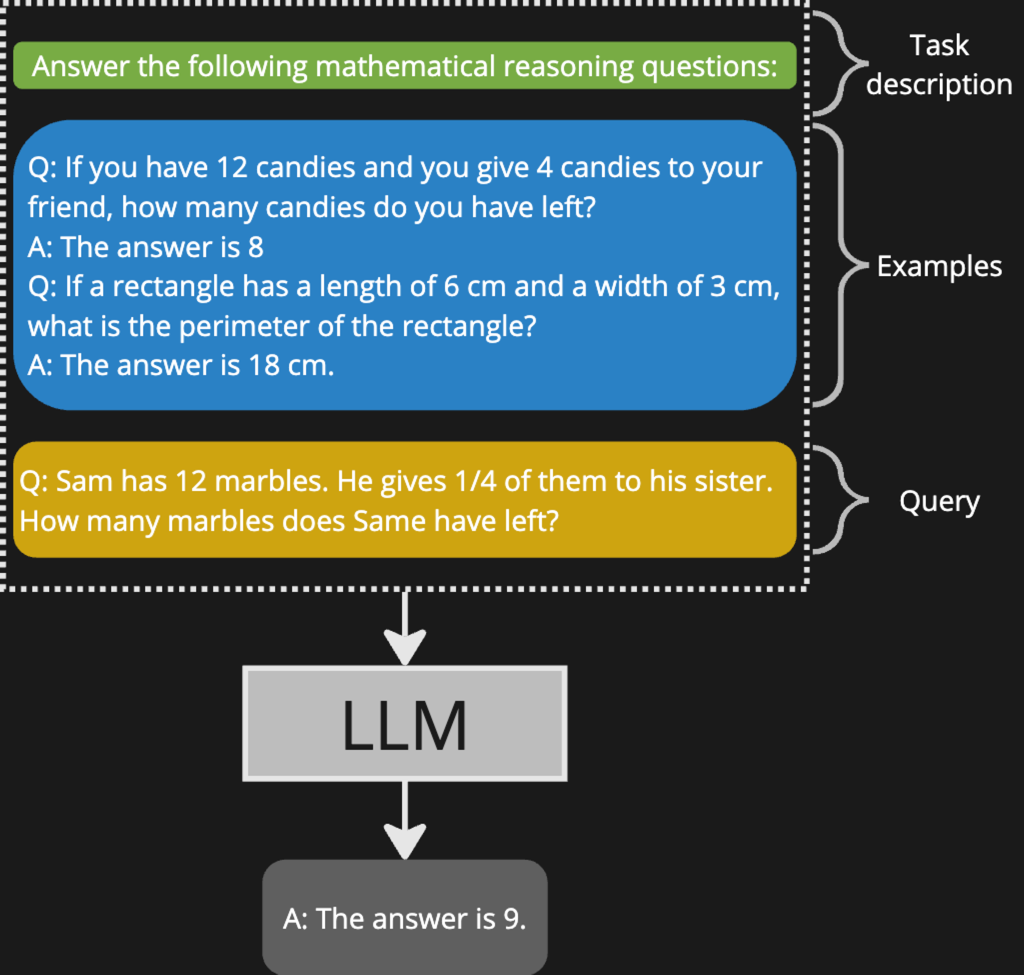
\includegraphics[width=\textwidth]{icl}
	\caption{In-context learning contrasted with traditional fine-tuning. Source: \textcite{brown2020language}}
	\label{fig:in-context-learning}
\end{figure}
ICT consists of the task description and/or a few examples of the task as demonstrations combined in a specific order to form natural language prompts with specifically designed templates~\cite{brown2020language}.
Finally, the test instance is appended to the prompt to form the input for LLMs to generate the output.

Based on task demonstrations, LLMs can learn to perform a new task without explicit gradient update.
Formally, the in-context learning task can be defined as follows:
\begin{equation}
	LLM(I, \underbrace{f(x_1, y_1), \dots, f(x_k, y_k)}_\text{demonstrations}, \underbrace{f(x_{k+1}}_\text{input}, \underbrace{\uline{~~~}}_\text{answer})) \rightarrow \hat{y}_{k+1}
	\label{eq:ict}
\end{equation}
where $I$ is a task description, $f(x_i, y_i)$ function that converts task demonstration to natural language, $x_{k+1}$ is a new input query, $\hat{y}_{k+1}$ is the prediction of the output generated, and the actual answer $y_{k+1}$ is left as a blank to be predicted by the LLM\@.

\begin{figure}[h!]
	\centering
	\resizebox{\textwidth}{!}{
		\begin{forest}
			forked edges,
			for tree={
					grow=east,
					reversed=true, % reverse the direction of growth
					anchor=base west, % align text to the west
					parent anchor=east,
					child anchor=west,
					base=left,
					font=\small,
					rectangle,
					draw,
					align=left,
					s sep=3mm, % sibling distance
					l sep=10mm, % level distance
					inner xsep=3mm, % text padding horizontal
					inner ysep=1mm  % text padding vertical
				}
				[In-context Learning
						[Inference
								[Scoring Function
										[{Channel prompt tuning~\cite{min2022metaicl},\\
													kNN-Prompting~\cite{xu2023knn}}]
								]
								[Demonstration Designing
										[Organization
												[Selecting
														[{KATE~\cite{liu2022good}, \\
																	EPR~\cite{rubin2022learning}, \\
																	PPL~\cite{gonen2022demystifying}, \\
																	SG-ICL~\cite{kim2022self}, \\
																	Self Adaptive~\cite{wu2022selfadaptive}, \\
																	MI~\cite{sorensen2022information}, \\
																	Q-Learning~\cite{zhang2022active}, \\
																	Informative Score~\cite{li2023finding}, \\
																	Topic~\cite{wang2023large}, \\
																	UDR~\cite{li2023finding}}]
												]
												[Ordering
														[{GlobalE\&LocalE~\cite{lu2022fantastically}}]
												]
										]
										[Formatting
												[Instruction
														[{Instruction Induction~\cite{honovich2022instruction}, \\
																	APE~\cite{zhou2022least}, \\
																	Self-Instruct~\cite{wang2022selfinstruct}}]
												]
												[Reasoning Steps
														[{CoT~\cite{wang2022selfinstruct}, \\
																	Complex CoT~\cite{fu2022complexity}, \\
																	AutoCoT~\cite{zhang2022automatic}, \\
																	Self-Ask~\cite{press2022train}, \\
																	MoT~\cite{li2023mot}, \\
																	SuperICL~\cite{xu2023small}, \\
																	iCAP~\cite{wang2022iteratively}, \\
																	Least-to-Most Prompting~\cite{zhou2022least} }]
												]
										]
								]
						]
						[Training
								[Warmup
										[Self-supervised In-context Training
												[{Self-supervised ICL~\cite{chen2022improving}, \\
															PICL~\cite{gu2023pretraining}}]
										]
										[Supervised In-context Training
												[{MetaICL~\cite{min2022metaicl}, \\
															OPT-IML~\cite{iyer2022opt}, \\
															FLAN~\cite{wei2022fine}, \\
															Super-NaturalInstructions~\cite{wang2022super}, \\
															Scaling Instruction~\cite{chung2022scaling}, \\
															Symbol Tuning~\cite{wei2023symbol}}]
										]
								]
						]
				]
		\end{forest}
	}
	\caption{Taxonomy of in-context learning. The training and the inference stage are two main stages for ICL. During the training stage, existing ICL studies mainly take a pre-trained LLM as the backbone and optionally warm up the model to strengthen and generalize the ICL ability. Towards the inference stage, the demonstration designing and the scoring function selecting are crucial for the ultimate performance. Source: \textcite{dong2023survey}}
	\label{fig:icl-taxonomy}
\end{figure}

Since ICL's performance heavily relies on demonstrations, it is important to design them properly in the prompts.
The three main aspects are a direct consequence of what is defined in Equation~\ref{eq:ict}: how to select the task demonstrations, convert them into natural language, and arrange demonstrations in a reasonable order.

Different training strategies enhance ICL capabilities, improving performance across various tasks without specific task optimization during the pre-training phase (see Figure~\ref{fig:icl-taxonomy} under the Training branch).
Main approaches include Supervised In-context Training, such as MetaICL\footnote{Meta-training for InContext Learning} and Symbol Tuning, and Self-supervised In-context Training, such as Self-supervised ICL and PICL~\cite{dong2023survey}.

MetaICL~\cite{min2022metaicl} proposed to continually train LLMs on a wide range of tasks\footnote{Classification, question answering,
	natural language inference, paraphrase detection and more} with demonstration examples.
This approach is related to other works that use multi-task learning for better zero-shot performance at test time~\cite{min2022metaicl}.
However, MetaICL is distinct as it allows learning new tasks from k examples alone, without relying on task reformatting (e.g., reducing everything to question answering)
or task-specific templates (e.g., converting different tasks to a language modelling problem).
MetaICL is based on the core idea of in-context learning by conditioning on training examples (i.e., explicitly training on an in-context learning objective).

Symbol Tuning~\cite{wei2023symbol} instead fine-tunes language models on in-context input-label pairs, substituting natural language labels (e.g., "positive/negative sentiment") with arbitrary symbols (e.g., "foo/bar").
As a result, symbol tuning demonstrates an enhanced capacity to utilize in-context information for overriding prior semantic knowledge.
Compared to MetaICL, which constructs several demonstration examples for each task, instruction tuning mainly considers an explanation of the task and is easier to scale up.

Self-supervised ICL leverages raw corpora to generate input/output pairs as training data, while PICL also utilizes raw corpora but employs a simple language modelling objective, promoting task inference and execution based on context.
PICL has shown to be more effective in zero-shot settings and task generalization~\cite{dong2023survey}.

Effective demonstration design is crucial, involving selecting and ordering examples or using instruction induction and reasoning steps (as shown in Figure~\ref{fig:icl-taxonomy} under the Inference/ Demonstration Designing branch).
The selection aims to choose good examples for ICL using unsupervised\footnote{Based on pre-defined metrics} or supervised methods.
For example, KATE~\cite{liu2022good} and EPR~\cite{rubin2022learning} select demonstrations based on similarity.
The ordering of the selected demonstrations is also an important aspect of demonstration design.
\textcite{lu2022fantastically} have proven that order sensitivity is a common problem and affects various models.
To address this problem, studies have proposed several training-free methods for ordering demonstrations.
\textcite{liu2022good} sorted examples based on similarity, while GlobalE\&LocalE~\cite{lu2022fantastically} orders demonstrations based on global and local entropy.

A common representation of demonstrations is concatenating examples $(x_1, y_1), \cdots, (x_k, y_k)$ with a template T directly.
However, this approach may not be optimal for all tasks, i.e.\ when the task is complex or requires multiple steps such as math word problems and common-sense reasoning.
In those cases, it's not easy to learn the mapping from $x_i$ to $y_i$ with only $k$ demonstrations.
Template engineering has been studied in \textcite{liu2021pretrain, liu2022good} to generate task-specific templates.
Some researchers have proposed designing a better format for demonstrations by describing tasks with instructions I and adding intermediate reasoning steps between examples $(x_i, y_i)$.
Instructions depend heavily on human input, but they can be generated automatically as shown in \textcite{honovich2022instruction} given several demonstration examples.
\textcite{zhou2023large} proposed APE for automatic instruction generation and selection.
To further improve the quality of the automatically generated instructions, \textcite{wang2022selfinstruct} proposed Self-Instruct, which is able to get rid of its own generations.

The approach of adding intermediate reasoning steps between examples introduced in \textcite{wang2023large} is also called Chain-of-Thought prompting.
We will delve into Chain-of-Thought prompting in the next Section~\ref{sec:chain-of-thought}.

At the inference stage, ICL operates without explicit updates, focusing on task recognition and learning through demonstrations.
Task recognition utilizes pre-trained knowledge to solve tasks identified in the demonstrations.
A Probably Approximately Correct (PAC)~\cite{wies2023learnability} framework has been proposed to evaluate ICL’s learnability, suggesting that LLMs can recognize tasks from minimal inputs.

Task learning, on the other hand, involves LLMs learning new tasks through demonstrations, akin to implicit fine-tuning through the attention mechanism, which generates meta-gradients.
With the examples provided in ICL, LLMs can implement learning algorithms such as gradient descent or directly compute the closed-form solution to update these models during forward computation.
Under this explanation framework, it has been shown that LLMs can effectively learn simple linear functions and even some complex functions like decision trees with ICL~\cite{akyurek2022what}.
Different model scales exhibit distinct capabilities; smaller models are adept at task recognition, while larger models (at least 66 billion parameters) are necessary for task learning~\cite{pan2023what}.

\begin{table}[h!]
	\centering
	\small
	\begin{tabularx}{0.8\textwidth}{lXccc}
		\toprule
		\textbf{Scoring Function} & \textbf{Target}              & \textbf{Efficiency} & \textbf{Task Coverage} & \textbf{Stability} \\
		\midrule
		Direct                    & $\mathcal{M}(y_j \mid C, x)$ & +++                 & +                      & +                  \\
		PPL                       & PPL($S_j$)                   & +                   & +++                    & +                  \\
		Channel                   & $\mathcal{M}(x \mid C, y_j)$ & +                   & +                      & ++                 \\
		\bottomrule
	\end{tabularx}
	\caption{Summary of different scoring functions.}
	\label{tab:scoring-functions}
\end{table}

The last piece of ICL is the scoring function, which decides how to transform the LLMs' predictions into an estimation of the likelihood of a specific answer.
A direct estimation method adopts the conditional probability of candidate answers and selects the higher probability as the final answer~\cite{brown2020language}.
However, this method poses some restrictions on the template design. For example, the answer tokens should be placed at the end of the input sequences.
Perplexity (PPL) is another commonly used metric that computes the PPL of the entire input sequence:
\begin{equation}
	S_j = \{C,s(x,y_i,I)\}
	\label{eq:ppl}
\end{equation}
where C are the tokens of the demonstration examples, $x$ is the input query, and $y_i$ is the candidate label.
As PPL is a global metric (i.e., it considers the entire input sequence), it removes the limitations of token positions but requires extra computation time.
In generation tasks such as machine translation, ICL predicts the answer by decoding tokens with the highest sentence probability combined with diversity-promoting strategies such as beam search or Top-p and Top-k~\cite{holzman2020curious} sampling algorithms.
\textcite{min2022noisy} proposed a channel scoring function that estimates the likelihood of the input query given the candidate answer\footnote{Compute the conditional
	probability in a reversed direction}, which is more efficient and stable than the direct estimation method.
In this way, language models are required to generate every token in the input, which could boost the performance under imbalanced training data regimes.
To calibrate the bias or mitigate the sensitivity via scoring strategies, some studies add additional calibration parameters to adjust the model predictions~\cite{zhao2021calibrate}.

\subsection{ICL performance and origins}
\label{subsec:icl-performance}

Knowing and understanding the factors that influence ICL can help to improve the performance of LLMs.
ICL has a close connection with instruction tuning (discussed in Section~\ref{subsec:instruction-tuning}) in that both utilize natural language to format the task or instances.
However, instruction tuning needs to fine-tune LLMs for adaptation, while ICL only prompts LLMs for utilization~\cite{survey}.
Furthermore, instruction tuning can enhance the ICL ability of LLMs to perform target tasks, especially in the zero-shot setting\footnote{Using only task descriptions}~\cite{chung2022scaling}.

\begin{table}[h!]
	\centering
	\small
	\begin{tabularx}{0.8\textwidth}{lX}
		\toprule
		\textbf{Stage} & \textbf{Factor}                                                                               \\
		\midrule
		\multirow{4}{*}{Pretraining}
		               & Pretraining corpus domain~\cite{shin2022effect}                                               \\
		               & Pretraining corpus combination~\cite{shin2022effect}                                          \\
		               & Number of model parameters~\cite{wei2022emergent, brown2020language}                          \\
		               & Number of pretraining steps~\cite{wei2022emergent}                                            \\
		\midrule
		\multirow{8}{*}{Inference}
		               & Label space exposure~\cite{min2022rethinking}                                                 \\
		               & Demonstration input distribution~\cite{min2022rethinking}                                     \\
		               & Format of input-label pairing~\cite{min2022rethinking,an2023how}                              \\
		               & Demonstration input-label mapping~\cite{min2022rethinking, yoo2022groundtruth, wei2023symbol} \\
		               & Demonstration sample ordering~\cite{lu2022fantastically}                                      \\
		               & Demonstration-query similarity~\cite{lu2022fantastically}                                     \\
		               & Demonstration diversity~\cite{an2023how}                                                      \\
		               & Demonstration complexity~\cite{an2023how}                                                     \\
		\bottomrule
	\end{tabularx}
	\caption{Summary of factors that have a relatively strong correlation to ICL performance. Source: \textcite{dong2023survey}}
	\label{tab:icl-factors}
\end{table}

There are several factors that have a relatively strong correlation to ICL performance, as shown in Table~\ref{tab:icl-factors}.
ICL ability may arise putting multiple corpora together in the pre-training stage, and the domain source is more important than the corpus size~\cite{shin2022effect}, while pre-train on corpora related to downstream tasks and models with lower perplexity does not always perform better in ICL~\cite{shin2022effect}.
\textcite{wei2022emergent} suggested that a pre-trained model suddenly acquires some emergent ICL abilities when it achieves a large scale of pretraining steps or model parameters, and \textcite{brown2020language} showed that the ICL ability grows as the parameters of LLMs increase from 0.1 billion to 175 billion.
At the inference stage, the properties of the demonstrations influence the ICL performance, such as the label space exposure, the format of input-label pairing, the ordering of demonstration samples, and the complexity of demonstrations~\cite{min2022rethinking, an2023how, lu2022fantastically}.
There are contrasting results on the impact of input-label mapping related to ICL~\cite{min2022rethinking, yoo2022groundtruth}.
An interesting finding is that, when a model is large enough, it will show an emergent ability to learn input-label mappings, even if the labels are flipped\footnote{Flipped-label ICL uses flipped targets, forcing the model to override semantic priors in order to follow the in-context exemplars. For example, in the sentiment analysis task, the label "Positive" becomes "Negative" in ICL context and viceversa} or semantically-unrelated\footnote{The labels are semantically unrelated to the task(e.g., for sentiment analysis, it uses “foo/bar” instead of “negative/positive”)}~\cite{wei2023larger}.
Some general validated factors for the ICL demonstrations are that they should be diverse, simple, and similar to the test example in terms of the structure~\cite{an2023how}.
\textcite{lu2022fantastically} indicated that the demonstration sample order is also an important factor.
\textcite{liu2022good} found that the demonstration samples with closer embeddings to the query samples usually perform better than those with farther embeddings.

The reasons for the ICL ability have been investigated from different perspectives.
Focusing on the pretraining data distribution, \textcite{chan2022data} showed that the ICL ability is driven by data distributional properties.
The ICL ability emerges when the training data have examples appearing in clusters and have enough rare classes.
\textcite{xie2022an} explained ICL as implicit Bayesian inference and constructed a synthetic dataset to prove that the ICL ability emerges when the pretraining distribution follows a mixture of hidden Markov models.
Under the learning mechanism, the ICL ability is explained by the ability of Transformers to encode effective learning algorithms to learn unseen linear functions according to demonstration samples, and encoded learning algorithms can achieve a comparable error to that from the least squares estimator~\cite{garg2023transformers}.
Also \textcite{li2023transformers} showed the ability of Transformers to implement a proper function class through implicit empirical risk minimization for the demonstrations.
From an information-theoretic perspective, \textcite{hahn2023theory} showed an error bound for ICL under linguistically motivated assumptions to explain how next-token prediction can bring about the ICL ability.
Another series of works attempted to build connections between ICL and gradient descent and found that Transformer-based in-context learners can implement standard fine-tuning algorithms implicitly~\cite{akyurek2022what, vonoswald2023transformers, li2023transformers}.
Looking at functional components, \textcite{olsson2022incontext} found indirect evidence that "Induction heads"\footnote{attention heads that implement a simple algorithm to complete token sequences like $[A][B] \dots [A] \Rightarrow [B]$} might constitute the mechanism for the majority of all ICL in large transformer models.

In-context learning (ICL) evaluation spans traditional tasks and newly proposed challenging tasks, and it provides open-source tools for standardized evaluation.
ICL has been tested against established benchmarks, such as SuperGLUE and SQuAD, with mixed results.
GPT-3, for example, exhibited comparable performance to state-of-the-art fine-tuning on some tasks within SuperGLUE but lagged in most natural language understanding tasks.
Scaling the number of demonstration examples has shown potential but has yet to bridge the gap fully between ICL and traditional fine-tuning methods~\cite{brown2020language, hao2022structured}.

New benchmarks have been introduced to assess the capabilities of large language models (LLMs) beyond traditional fine-tuning.
The BIG-Bench and BIG-Bench Hard focus on tasks ranging from linguistics to social behaviours, with models outperforming human raters on many of these tasks~\cite{srivastava2023imitation, suzgun2022challenging}.
OPT-IML Bench has been designed to evaluate the generalization capabilities of LLMs across various held-out categories, emphasizing the model's generalization capabilities~\cite{iyer2022opt}.
OpenICL has been developed to provide a flexible and unified framework for ICL evaluation.
This toolkit supports different LLMs and tasks, enabling consistent implementation and evaluation of ICL methods across various studies~\cite{wu2023openicl}.

The application of In-Context Learning (ICL) has transcended the domain of natural language processing (NLP), influencing research in various modalities such as visual tasks, vision+language integration, and speech.
Visual In-Context Learning explores how models generalize learned visual concepts to new, unseen tasks by leveraging contextual demonstrations in a manner akin to NLP-based ICL. Techniques such as image patch infilling and the training of models like masked autoencoders (MAE) exemplify this approach~\cite{bar2022visual}.
Noteworthy models like Painter and SegGPT have been developed to handle multiple tasks or integrate various segmentation tasks into a single framework~\cite{wang2023images, wang2023seggpt}.
The Prompt Diffusion model introduced by \textcite{wang2023incontext} represents a pioneering effort in diffusion-based models displaying ICL capabilities, particularly when guided by textual prompts~\cite{wang2023incontext}.
The integration of visual contexts with linguistic models has led to significant advancements in vision-language tasks.
Models such as Frozen and Flamingo have demonstrated the feasibility of multi-modal, few-shot learning by combining vision encoders with large language models (LLMs).
These models effectively perform ICL on multi-modal tasks when trained on large-scale multi-modal web corpora~\cite{tsimpoukelli2021frozen, alayrac2022flamingo}.
Kosmos-1 and METALM further extend these capabilities by demonstrating strong performance across various vision-language tasks, underpinned by a semi-causal language modelling objective~\cite{huang2023language, hao2022language}.

\subsection{ICL future research}
\label{subsec:icl-future}

Future research in ICL is expected to focus on several key areas, including the optimization of pretraining objectives, the distillation of ICL abilities, the enhancement of ICL robustness, the improvement of ICL efficiency and scalability, the updating of knowledge within LLMs, the augmentation of models, and the expansion of ICL into multi-modal domains~\cite{dong2023survey}.
Optimizing pretraining objectives to better align with ICL requirements could enhance model capabilities for ICL applications.
Introducing intermediate tuning phases and tailoring pretraining objectives to better align with ICL requirements could bridge this gap and enhance model capabilities for ICL applications~\cite{shin2022effect}.
An important goal is to distil ICL capabilities from larger models to smaller, more efficient ones, potentially enabling the deployment of ICL in resource-constrained environments~\cite{magister2022teaching}.
Another area of improvement is the robustness of ICL, which is highly susceptible to the format and permutation of demonstrations~\cite{zhao2021calibrate, lu2022fantastically}, without compromising accuracy or efficiency~\cite{chen2024relation}.

A more theoretical understanding of ICL's mechanisms could lead to more robust implementations.
Moreover, the scalability of ICL is constrained by the input limitations of language models and the computational cost associated with large numbers of demonstrations.
Innovative strategies like structured prompting~\cite{hao2022structured} and dynamic prompting~\cite{wang2023efficient} are being explored to address these challenges.
The development of models with extended context capabilities~\cite{li2023contextual} indicates significant potential for progress in this area.
Finally, the expansion of ICL into multi-modal domains is expected to yield new insights and applications, particularly in the fields of vision and speech~\cite{dong2023survey}.


\section{Chain-of-Thought}
\label{sec:chain-of-thought}

Chain-of-Thought (CoT) prompting is an enhanced strategy developed to augment the performance of large language models (LLMs) on complex reasoning tasks such as arithmetic, commonsense, and symbolic reasoning~\cite{wei2022chain, miao2021diverse, talmor2019commonsenseqa}.
This method integrates intermediate reasoning steps within the prompts, thereby providing a more structured path towards the solution.
\begin{figure}[h!]
	\centering
	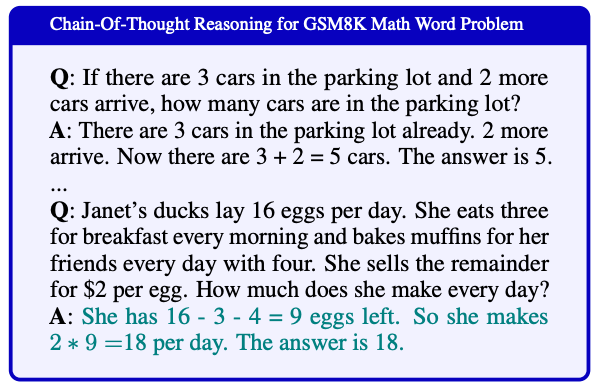
\includegraphics[width=0.6\textwidth]{cot-reasoning}
	\caption{Chain-of-Thought reasoning for GSM8k math word problem. The prompt is coloured black, and the reasoning path produced by the language model is coloured teal. This reasoning path contains two reasoning steps. Source: \textcite{li2022making}}
	\label{fig:cot-reasoning}
\end{figure}
To some extent, CoT can be considered a special case of ICL, as it involves the generation of prompts with a series of intermediate reasoning steps (Figure~\ref{fig:chain-of-thought}), but the ordering of demonstrations in this case has a s relatively minor impact on the performance of LLMs~\cite{wei2022chain}.

\textcite{wei2022chain, wang2022self} have shown that language models, when large enough (i.e., \textgreater 100 billion parameters), can learn to perform complex reasoning tasks through CoT prompting without explicit task-specific~\cite{wei2022emergent}.

\begin{figure}[h!]
	\centering
	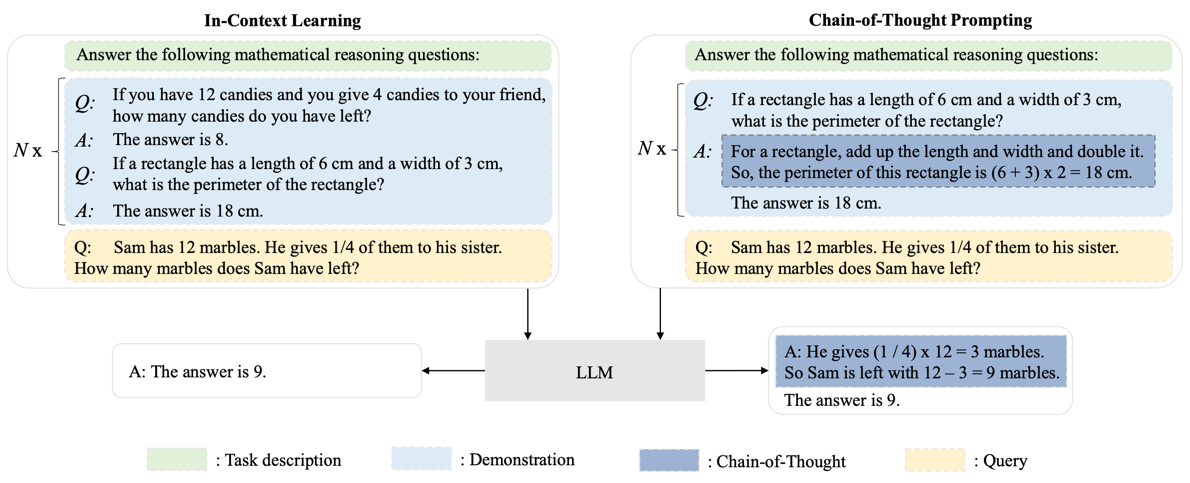
\includegraphics[width=\textwidth]{icl-vs-cot}
	\caption{A comparative illustration of in-context learning (ICL) and chain-of-thought (CoT) prompting. ICL prompts LLMs with a natural language description, several demonstrations, and a test query, while CoT prompting involves a series of intermediate reasoning steps in prompts. Source: \textcite{survey}}
	\label{fig:chain-of-thought}
\end{figure}

CoT can be effectively combined with In-context Learning (ICL) in both few-shot and zero-shot settings:
\begin{itemize}
	\item \textbf{Few-shot CoT.} {In the few-shot scenario, CoT augments standard input-output pairs with intermediate reasoning steps.
		      The design of CoT prompts is crucial; incorporating diverse and complex reasoning paths has been shown to significantly boost LLM performance.
		      An automated approach, Auto-CoT, facilitates the generation of CoT sequences without manual effort by clustering and selecting representative questions~\cite{zhang2022automatic}.
	      }
	\item \textbf{Zero-shot CoT.} {Unlike its few-shot counterpart, zero-shot CoT does not rely on annotated demonstrations.
		      Instead, it generates reasoning steps directly from a prompt, significantly improving performance when scaled to larger models.
		      This approach was pioneered by models like Flan-T5, which demonstrated improved zero-shot performance through instruction tuning on CoT annotations~\cite{chung2022scaling}.
	      }
\end{itemize}

\begin{figure}[h!]
	\centering
	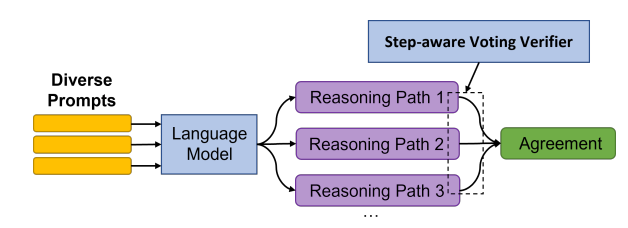
\includegraphics[width=0.6\textwidth]{diverse}
	\caption{The DIVERSE approach for CoT. Source: \textcite{li2022making}}
	\label{fig:diverse}
\end{figure}

To apply these strategies effectively, it is essential to design CoT prompts that guide the model through the reasoning process.
In \textcite{li2022making}, the authors have shown that using diverse CoTs (i.e., prompts with multiple reasoning paths for each problem) can significantly enhance the performance of LLMs on complex reasoning tasks.
The proposed method, DIVERSE\footnote{\textbf{Di}verse \textbf{Ve}rifier on \textbf{R}easoning \textbf{S}t\textbf{e}p}, generates diverse CoTs by leveraging a self-ensemble approach that alternates between selection and inference.
It has three main components: first, it generates diverse prompts to explore different reasoning paths for the same question; second, it uses a verifier to filter out incorrect answers based on a weighted voting scheme; and third, it verifies each reasoning step individually instead of the whole chain (Figure ~\ref{fig:diverse}).
In the first step, the model generates multiple reasoning paths for each question, which are then used to generate diverse prompts following the idea that \textit{"All roads lead to Rome"}.
As an improvement of \textcite{wang2022self}, DIVERSE selects $M_1$ different prompts for each question and $M_2$ reasoning paths for each prompt, resulting in $M_1 \times M_2$ diverse prompts.
Then, the verifier takes a question and a candidate's reasoning path and outputs the probability that the reasoning path leads to the correct answer.
Different predictions are aggregated using a \textit{voting verifier} to obtain the final prediction:
\begin{equation}
	\hat{y} = \underset{y}{\text{arg max}} \sum_{i=1}^{M_1} \textbf{1}_{y = y_{i}} \cdot f(\textbf{x}_i, \textbf{z}_i, \textbf{y}_i)
	\label{eq:diverse}
\end{equation}
where $\textbf{1}_{y = y_{i}}$ is an indicator function that equals 1 if $y = y_{i}$, and $f(\cdot)$ is the probability produced by the verifier.

\begin{figure}[h!]
	\centering
	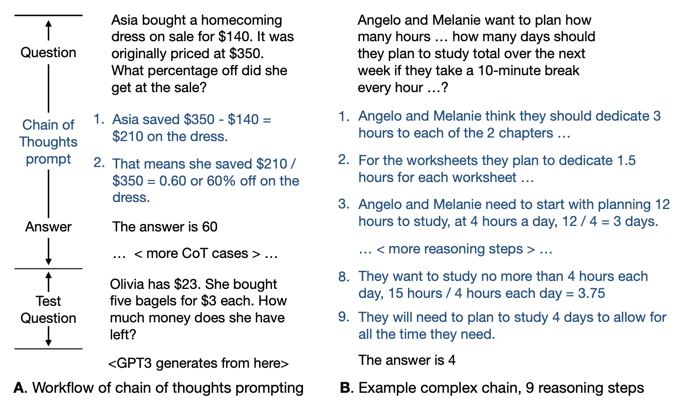
\includegraphics[width=0.8\textwidth]{cot-complex-chain}
	\caption{\textbf{A}: Chain of thoughts (in blue) are intermediate reasoning steps towards a final answer. The input of CoT prompting is a stack of a few (often 8) CoT cases before a test question. Then, the language model will continue generating an output CoT for the test question. \textbf{B}: Chains of harder reasoning complexity are chains with more reasoning steps (9 steps in this case, v.s. only 2 steps in subfigure A). Source: \textcite{fu2022complexity}}
	\label{fig:cot-complex-chain}
\end{figure}

Another intuitive idea is that prompting with more complex reasoning steps (i.e., chains with more reasoning steps) is more likely to elicit the reasoning ability of LLMs~\cite{fu2022complexity}, which can result in generating correct answers (Figure~\ref{fig:cot-complex-chain}).
There are other complexity indicators than the number of reasoning steps, such as question lengths or the length of the underlying formula for solving a given problem, but improvements in performance are consistent across various complexity indicators.
Consequently, for datasets not annotated with reasoning steps, question length can be used as a proxy for complexity to generate CoT prompts.
In that way, it is possible to annotate only the identified few-shot instances, thus reducing the annotation cost~\cite{fu2022complexity}.
To exclude complexity correlated factors, \textcite{fu2022complexity} proposed prompts evaluation:
\begin{itemize}
	\item \textbf{Simpler examples but the same total number of reasoning steps.} {For instance, comparing 24 cases that each require 3 reasoning steps with 8 cases that each require 9 reasoning steps, both resulting in a total of 72 steps.}
	\item \textbf{Prompts of the longest lengths but not necessarily the most steps.} {This ensures that the length itself is not the only factor being assessed.}
\end{itemize}
It turned out that the complexity of reasoning steps is the most important factor for the performance of LLMs on complex reasoning tasks~\cite{fu2022complexity}.
\begin{figure}[h!]
	\centering
	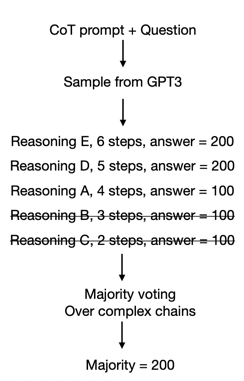
\includegraphics[width=0.2\textwidth]{cot-complexity}
	\caption{Complexity-based Consistency for CoT. During decoding, it samples N reasoning chains from the language model (N = 5 here) and takes the majority answer over the K (K = 3 here) most complex generated chains. Source: \textcite{fu2022complexity}}
	\label{fig:complexity}
\end{figure}
Complexity-based prompting can be further enhanced by using the output selection method called Complexity-based Consistency, alleviating the possibility that the model can take shortcuts during reasoning\footnote{Relying on spurious correlations that inevitably exist in the training data and are not related to the reasoning process as shown by \textcite{mudrakarta2018model, li2021why, sugawara2018makes}}.
The method explicitly promotes outputs with more complex reasoning chains at inference time, similar to the self-consistency practice in \textcite{wang2022self}.
A voting mechanism is used to select the final output among top K complex reasoning chains, as shown in Figure~\ref{fig:complexity}.

\begin{figure}[h!]
	\centering
	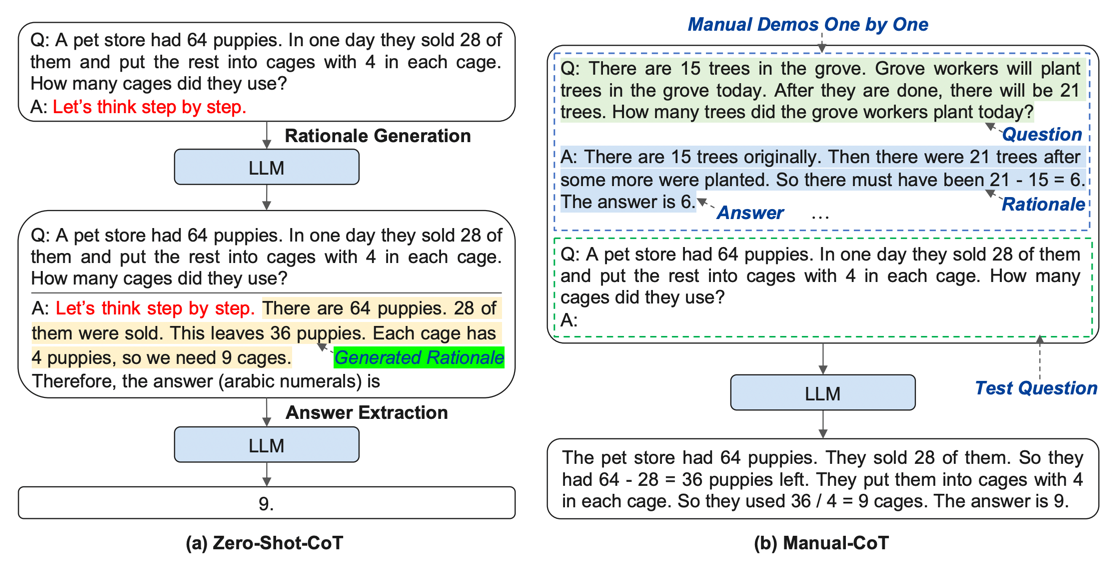
\includegraphics[width=\textwidth]{cot-zero}
	\caption{Zero-Shot-CoT~\cite{kojima2023large} (using the "Let’s think step by step" prompt) and Manual-CoT\cite{wei2022chain} (using manually designed demonstrations one by one) with example inputs and outputs of an LLM. Source: \textcite{zhang2022automatic}}
	\label{fig:zero-shot-cot}
\end{figure}

Previously mentioned methods rely on two major paradigms: Zero-Shot-CoT and Manual-CoT\@.
Zero-Shot-CoT is a task-agnostic paradigm that generates reasoning steps directly from the prompt, eliminating the need for annotated CoT datasets~\cite{kojima2023large}, adding a single prompt like "Let’s think step by step" after the test question to facilitate the reasoning chains in LLMs.
On the other hand, Manual-CoT uses manually designed demonstrations one by one, which can be expensive and time-consuming to create~\cite{wei2022chain}.
Since this prompting paradigm is task-agnostic and does not need input-output demonstrations, it is called Zero-Shot-CoT (left of Figure~\ref{fig:zero-shot-cot}).
With Zero-Shot-CoT, LLMs have shown to be decent zero-shot reasoners.

The other paradigm is few-shot prompting with manual reasoning demonstrations one by one~\cite{wei2022chain}.
Each demonstration has a question and a reasoning chain.
A reasoning chain is composed of a rationale (a series of intermediate reasoning steps) and an expected answer.
With all the demonstrations being manually designed, this paradigm is referred to as Manual-CoT (right of Figure~\ref{fig:zero-shot-cot}).

To mitigate the effect of reasoning chain mistakes from Zero-Shot-CoT, \textcite{zhang2022automatic} proposed the use of Auto-CoT, a method that generates demonstrations automatically since their diversity is crucial for the performance of LLMs.
It consists of two main components: a clustering algorithm that groups similar questions together and a representative selection algorithm that selects the most representative questions from each cluster.
The overall procedure is illustrated in Figure~\ref{fig:auto-cot}.
\begin{figure}[h!]
	\centering
	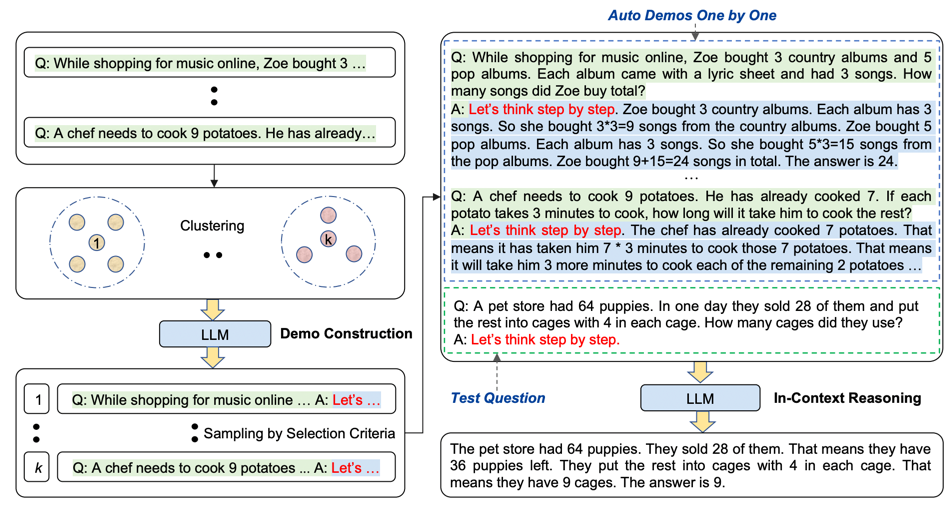
\includegraphics[width=\textwidth]{auto-cot}
	\caption{demonstrations (on the right) are automatically constructed one by one (total: k) using an LLM with the “Let’s think step by step” prompt. Source: \textcite{zhang2022automatic}}
	\label{fig:auto-cot}
\end{figure}
Diversity-based clustering may mitigate misleading by similarity effects\footnote{The retrieved demonstration questions are similar to the test question and ask "how long will it take him to cook \underline{the rest}?" The reasoning chains generated by Zero-Shot-CoT produce answers regarding "the total of" instead of "the rest". Following the demonstrations, the component that retrieves the top-k similar questions -- called Retrieval-Q-CoT -- also fails by misunderstanding the meaning of "the rest".}, and the representative selection algorithm can select the most representative questions from each cluster is used as demonstrations to generate reasoning chains for the test question.
Auto-CoT has shown to be effective in generating diverse reasoning chains and improving the performance of LLMs on arithmetic and symbolic reasoning~\cite{zhang2022automatic}.

\subsection{CoT performance and origins}
\label{subsec:cot-performance}

CoT is an emergent ability~\cite{wei2022emergent}, so it has positive effects only on the performance of LLMs (\textgreater 10 billion parameters) but not on smaller models.
Moreover, CoT is only effective for tasks that require step-by-step reasoning, such as arithmetic, commonsense, and symbolic reasoning~\cite{wei2022chain, miao2021diverse, talmor2019commonsenseqa}.
Whereas, for other tasks, CoT can be detrimental to the performance of LLMs with respect to standard prompting~\cite{wang2022rationale}, e.g., MNLI-m/mm, SST-2, and QQP from GLUE\cite{wang2018glue}.
It seems that the effectiveness of CoT is inversely proportional to the effectiveness of standard prompting~\cite{wei2022chain}.
Main prompting components, e.g., symbols, patterns, and text, have an impact on CoT.
It has been shown that pattern and text are essential for CoT performance, and removing them can lead to a significant drop in performance: text helps LLMs
to generate useful patterns, and patterns aid LLMs to understand tasks and generate texts that help solve them~\cite{madaan2022text}.

The origins of CoT ability are widely hypothesized to be elicited by training on code since those models have shown to be more effective in reasoning tasks~\cite{fu2022gptroadmap, liang2022holistic}.
Intuitively, code data is well organized with algorithmic logic and programming flow, which may be useful to improve the reasoning performance of LLMs. However, this hypothesis still lacks publicly reported evidence of ablation experiments (with and without training on code).
We'll try to address this gap in the next chapter~\ref{ch:capabilities}, by conducting a series of experiments to evaluate the effectiveness of training on code data for reasoning tasks.
In addition, instruction tuning seems not to be the main factor for CoT ability since the performance of LLMs on CoT tasks is not significantly improved by instruction tuning~\cite{chung2022scaling}.

\section{Planning for complex tasks}
\label{sec:planning}

ICL and CoT are two simple yet general strategies for solving various tasks.
However, they struggle with complex tasks that require long-term planning, such as mathematical word problems~\cite{qian2022limitations} and multi-hop question answering~\cite{bian2024chatgpt}.
Commonsense knowledge\footnote{It includes knowledge about the spatial,
	physical, social, temporal, and psychological aspects of the typical everyday life, as well as an awareness of social norms, beliefs, and values~\cite{liu2004conceptnet}.} is essential for NLP systems to understand and generate human-like language.
Main categories are summarized in \textcite{bian2024chatgpt}:
\begin{quote}
	\textbf{General commonsense} refers to knowledge that is widely shared and assumed to be true by most people, such as the sun rises in the east and sets in the west.\\
	\textbf{Physical commonsense} involves intuitive knowledge about the physical world, such as objects falling to the ground when dropped and water flowing downhill.\\
	\textbf{Social commonsense} involves knowledge about social norms, customs, and practices, such as it is polite to say "thank you" when
	making requests.\\
	\textbf{Science commonsense} involves knowledge about basic scientific principles, such as gravity pulling all objects on Earth to Earth’s centre.\\
	\textbf{Event commonsense} involves knowledge about the sequence of events and the causal relationships between them, such as if a glass is knocked over, the liquid inside will spill.\\
	\textbf{Numerical commonsense} involves knowledge about numbers, such as a human has two hands and ten fingers.\\
	\textbf{Prototypical commonsense} involves knowledge about typical or prototypical examples of concepts, such as a swallow is a kind of bird and a bird has wings.\\
	\textbf{Temporal commonsense} involves knowledge about time, such as travelling abroad requires a longer time than taking a walk.
\end{quote}
A list of commonsense QA datasets commonly used in evaluating LLMs is shown in Table~\ref{tab:dataset_examples}.
\begin{table}[h!]
	\small
	\centering
	\begin{tabularx}{\textwidth}{|l|l|X|}
		\hline
		Dataset       & Domain       & Example (Bold texts are the answers)                                                                                                                                                                                                                                     \\
		\hline
		CommonsenseQA & General      & Choose your answer to the question: Where are you likely to find a hamburger? \textbf{A. fast food restaurant}, B. pizza, C. ground up dead cows, D. mouth, E. cow circus                                                                                                \\
		\hline
		OpenBookQA    & General      & Choose your answer to the question: If a person walks in the opposite direction of a compass arrow they are walking A. west, B. north, C. east, \textbf{D. south}                                                                                                        \\
		\hline
		WSC           & General      & Choose sub-sentence A or B that completes the sentence: The trophy doesn't fit into the brown suitcase because A. the trophy is too small. \textbf{B. the suitcase is too small}.                                                                                        \\
		\hline
		PIQA          & Physical     & Choose one that is correct: A. \textbf{ice box will turn into a cooler if you add water to it}. B. ice box will turn into a cooler if you add soda to it.                                                                                                                \\
		\hline
		Social IQA    & Social       & Taylor taught math in the schools after studying to be a teacher. Choose the most suitable answer for the question: What does Taylor need to do before this? \textbf{A. get a certificate}, B. teach small children, C. work in a school                                 \\
		\hline
		ARC           & Science      & Choose your answer to the question: Which technology was developed most recently? \textbf{A. cellular telephone}, B. television, C. refrigerator, D. airplane                                                                                                            \\
		\hline
		QASC          & Science      & Choose your answer to the question: What is described in terms of temperature and water in the air? A. storms; \textbf{B. climate}; C. mass; D. seasonal; E. winter; F. density; G. length                                                                               \\
		\hline
		HellaSWAG     & Event        & Choose your answer to the question: We see a chair with a pillow on it. A. a man holding a cat does curling. B. a man holding a cat starts hitting objects on an item. C. a man holding a cat is wrapping a box. \textbf{D. a man holding a cat sits down on the chair}. \\
		\hline
		NumerSense    & Numerical    & a square is a shape with \textlangle mask\textrangle equally length sides. \textbf{(four)}                                                                                                                                                                               \\
		\hline
		ProtoQA       & Prototypical & Use simple words separated by commas to name something in your life that could cause you to lose weight. (\textbf{Eating less, exercising more, stress.})                                                                                                                \\
		\hline
		MC-TACO       & Temporal     & Select all feasible answers for the question: Carl Laemmle, head of Universal Studios, gave Einstein a tour of his studio and introduced him to Chaplin. At what time did Einstein return home? \textbf{A. 8:00 PM}; B. a second later; C. a hour later                  \\
		\hline
	\end{tabularx}
	\caption{Examples from commonsense QA datasets. Source: \textcite{bian2024chatgpt}}
	\label{tab:dataset_examples}
\end{table}
These datasets encompass domains like general, physical, social, science, event, numerical, prototypical, and temporal commonsense.
Table~\ref{tab:commonsense-results} shows the accuracy of GPT-3, GPT-3.5, and ChatGPT on these datasets.
\begin{table}[h!]
	\centering
	\small
	\begin{tabular}{|l|c|c|c|c|}
		\hline
		Dataset       & GPT-3 & Instruct GPT & ChatGPT       & Human \\
		\hline
		CommonsenseQA & 38    & \textbf{81}  & 74            & 88.9  \\
		OpenBookQA    & 22    & 65           & \textbf{73}   & 89.3  \\
		WSC           & 46    & \textbf{78}  & \textbf{78}   & 92.1  \\
		PIQA          & 48    & 77           & \textbf{78}   & 94.5  \\
		Social IQA    & 36    & \textbf{71}  & 62            & 86.9  \\
		ARC           & 27    & 88           & \textbf{94}   & --    \\
		QASC          & 25    & \textbf{75}  & 74            & 93.0  \\
		HellaSWAG     & 19    & 61           & \textbf{67}   & 95.7  \\
		NumerSense    & 45    & 63           & \textbf{79}   & 89.7  \\
		ProtoQA       & 67.3  & 84.6         & \textbf{94.2} & --    \\
		MC-TACO       & 20    & \textbf{53}  & 52            & 75.8  \\
		\hline
	\end{tabular}
	\caption{Evaluation results (accuracy) of large language models on commonsense QA datasets. Source: \textcite{bian2024chatgpt}}
	\label{tab:commonsense-results}
\end{table}
The ability of models to leverage commonsense is probably improved by instruction tuning and human alignment, looking at the results of Instruct GPT and ChatGPT versus GPT-3 in Table~\ref{tab:commonsense-results}.)
ChatGPT demonstrates strong capabilities in commonsense QA tasks but has limitations in identifying necessary knowledge.
It has been proved by evaluating answers generated by ChatGPT on questions from each commonsense QA dataset using the following prompt: "What knowledge is necessary for answering this question? \code{\{question\} \{answer choices(if applicable)\}}".
This means that LLMs are inexperienced problem solvers who rely on memorizing a large amount of information to cover the answers.

Even though we have seen surprising abilities of LLMs, \textcite{qian2022limitations} have shown additional limitations on certain basic symbolic manipulation tasks, such as copy, reverse and addition, particularly when dealing with repeating symbols\footnote{Copy example with repeating symbols \code{$\text{input:} \ldots 989894 \ldots \longrightarrow \text{answer:} \ldots 9894 \ldots$}} and OOD\footnote{Out-of-distribution refers to prompting the model to execute an operation on numbers with more digits with respect to numbers used for training. It demonstrates the ability to generalize on unseen data.} data.
To address these limitations, \textcite{qian2022limitations} have proposed a series of methods to improve the performance of LLMs on these tasks, such as positional markers, fine-grained computation steps, and combining LMs with callable programs for basic operations.
Positional markers\footnote{LMs have implicit positional markers embedded in the architecture. Most Transformer-based LMs encode the positional information into positional vectors and add each of
	them to the corresponding word vector. Explicit positional markers are added into input strings: \code{$\text{input:} \ldots 222 \ldots \longrightarrow \text{output:} \ldots \text{A} 2 \text{B} 2 \text{C} 2 \ldots$}.
	Essentially, adding explicit positional markers breaks the repeating numbers into a non-repeating input sequence.} and fine-grained computation steps\footnote{For example, in k-digit addition, the model is allowed to break it down into k simple 1-digit addition, and the model is allowed to generate k intermediate addition results to get the final answer.} provide some improvement with repeating symbols but not with OOD\@.
It clearly indicates the limitation of Transformers and pre-trained language models in induction.
Combining LMs with callable programs\footnote{A callable function \code{add(1,5)} can be invoked and return the result in text: \code{carry C: 0, result 6}} for basic operations shows potential but still relies on the LM's ability to locate tokens accurately.
The LM with tutor method
\footnote{A tutor shows every single step visually and sometimes calls an already learned sub-module to complete a task. Instead of providing a training example: \code{copy: 1 1 1 2 2 2 result: 1 1 1 2 2 2}, the tutor explicitly shows the model how to copy the input as follows: \code{rmov, end=F, cpy, rmov, end=F, cpy, \ldots , rmov, end=T.} where \code{rmov} is a function that moves the tape head to the right, \code{cpy} is a function that copies the current symbol, and \code{end=F} indicates that the end of the tape is not reached. One can relate the setting with a multiple tape Turing machine where state transition is conducted among the positions of tape heads and read/write operations. The Transformer is trained to learn such state transition, thus completing the programming of a Turing machine.} demonstrates each step of the task, significantly improving accuracy and handling OOD scenarios, effectively achieving 100\% accuracy on all tasks.

\subsection{Plan-based reasoning}
\label{subsec:plan-based}

Prompt-based planning has been proposed to break down complex tasks into simpler sub-tasks, and generate a plan of actions which can accomplish the task.
The general framework of prompt-based planning is shown in Figure~\ref{fig:planning}.

\begin{figure}[h!]
	\centering
	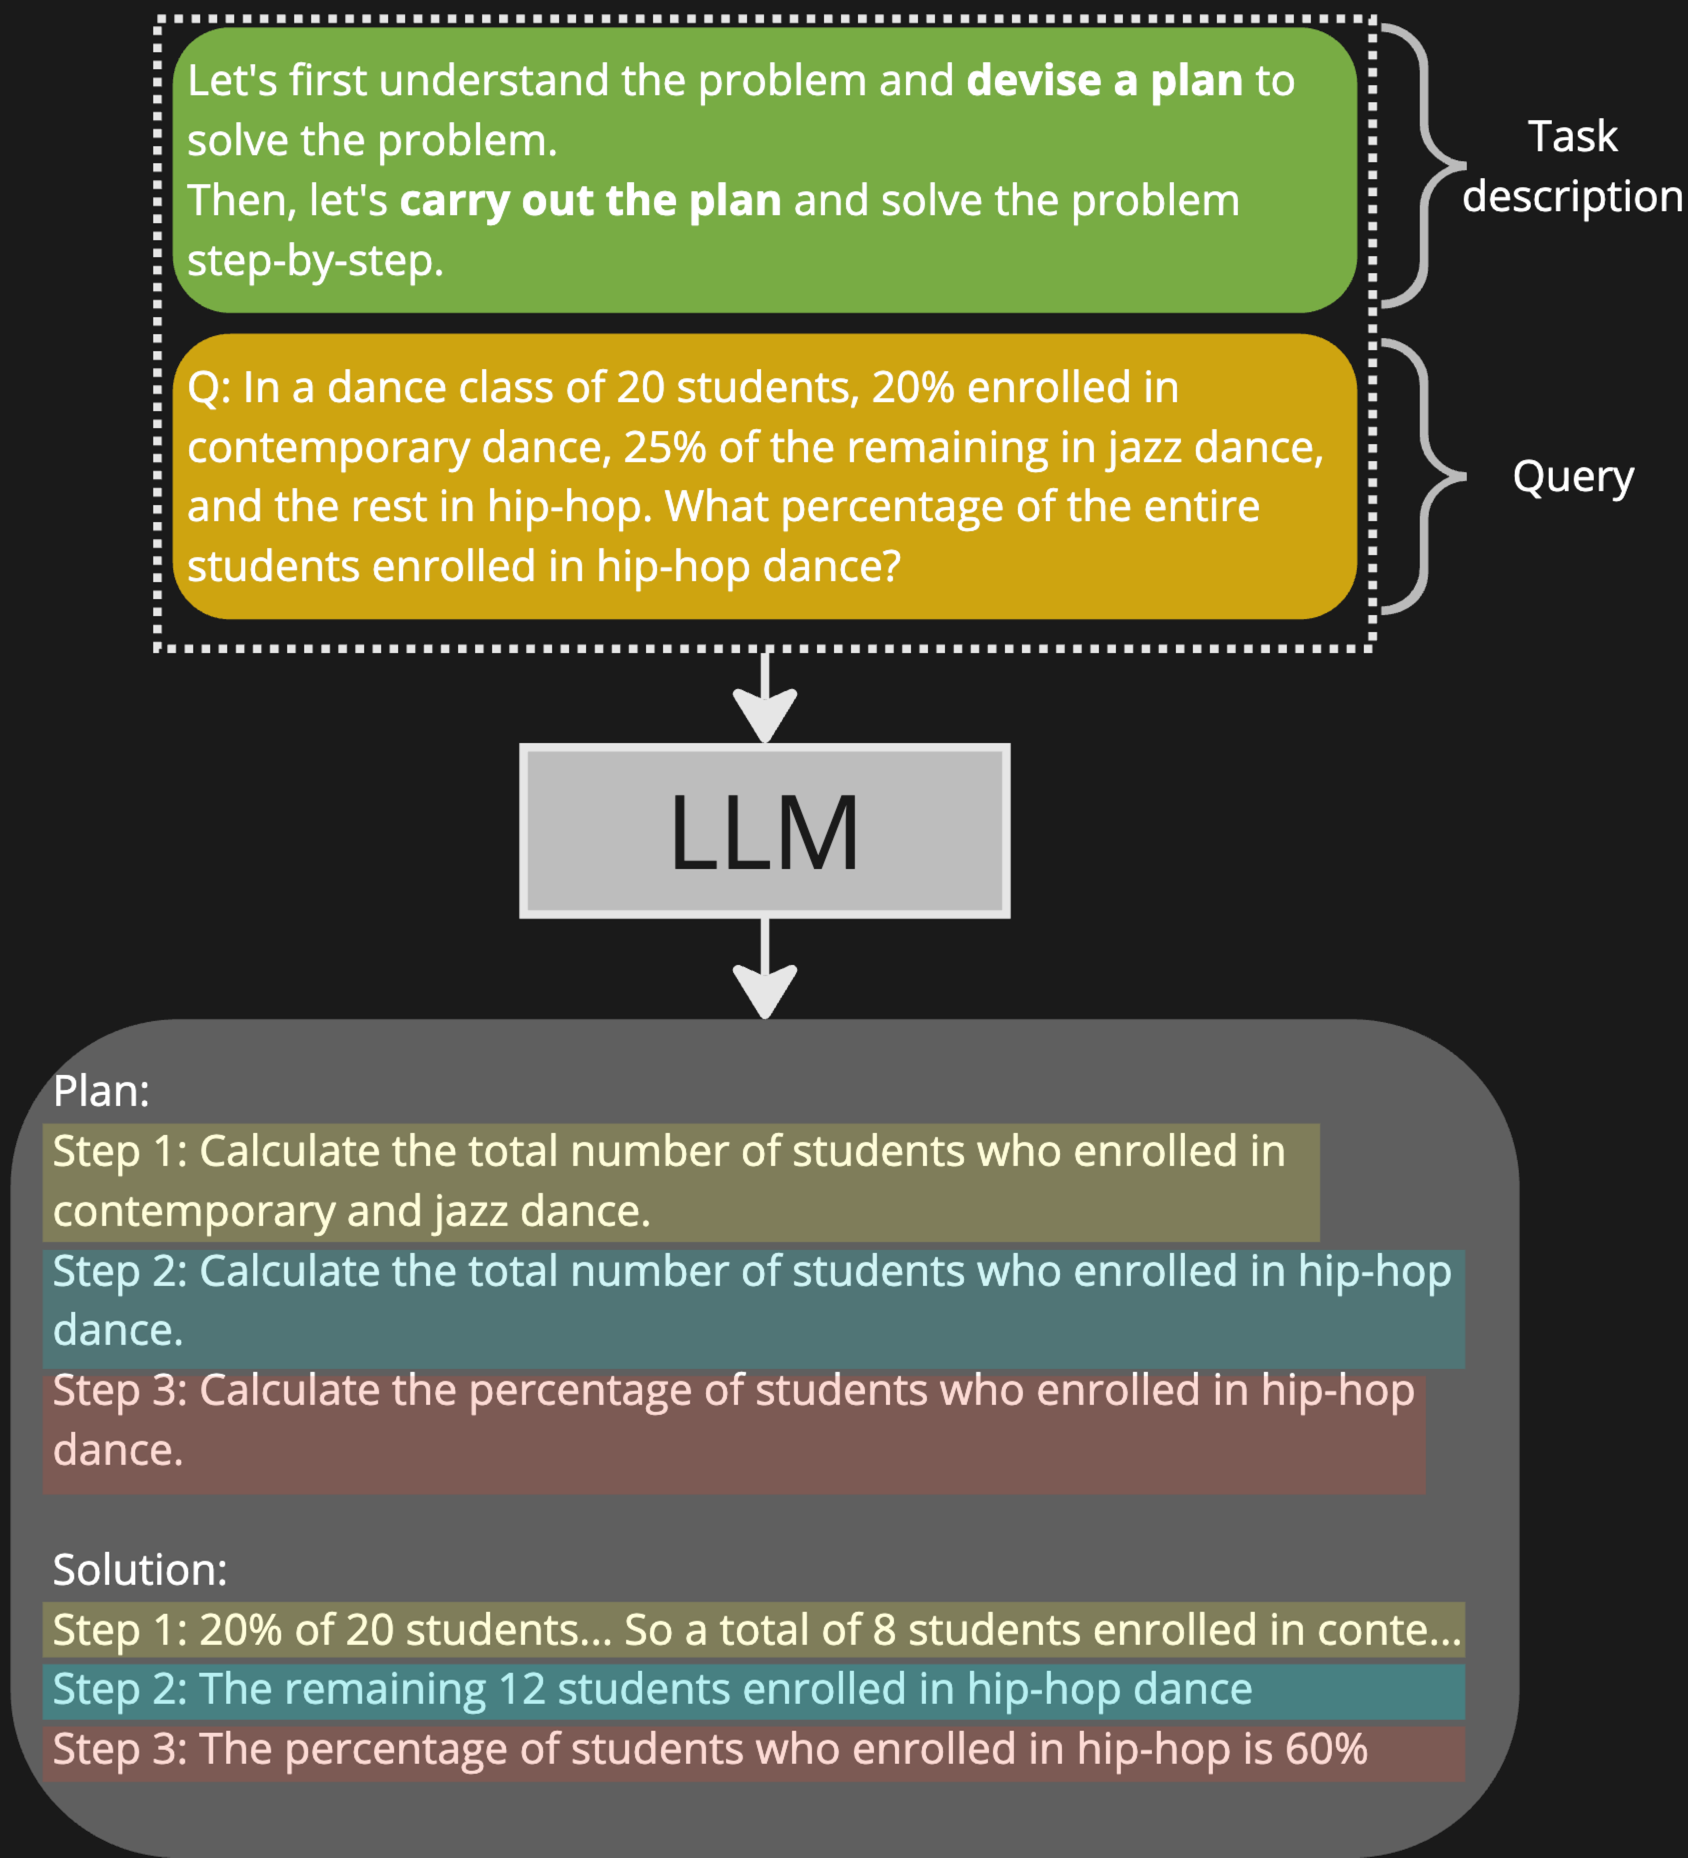
\includegraphics[width=0.8\textwidth]{planning}
	\caption{The general framework of prompt-based planning. Source: \textcite{survey}}
	\label{fig:planning}
\end{figure}

In this paradigm, there are three main components: the planner, the executor, and the environment\footnote{It's similar to Reinforcement Learning, where the planner is the agent, the executor is the policy, and the environment is the world, but the difference is that in RL they are typically interleaved in the agent, while in prompt-based planning they are separated}.
The first component is the planner, which generates a plan of action to solve the task.
The plan can be generated in various forms, e.g., natural language, symbolic, or programmatic~\cite{gao2022pal, zhou2022least}, that we will discuss in the next section~\ref{subsec:plan-based}.
The task planner can be enhanced with the memory mechanism, which stores intermediate results and reuses them in the future.

The plan executor is responsible for executing the plan generated by the planner.
It can be implemented as a separate LLM for textual tasks or as a program executor for programmatic tasks~\cite{wang2023plan, gao2022pal}.

The environment is the world where the task is executed, which can be set up as the LLM itself or an external system, e.g., a simulator or a virtual world like Minecraft~\cite{yao2023tree, wang2023voyager}.
The environment provides feedback to the task planner about the result of the actions, which can be used to update the plan, either in the form of natural language or from other multimodal signals~\cite{shinn2023reflexion, lu2023multimodal}

\subsubsection{Plan generation}
\label{subsubsec:plan-generation}

For solving complex tasks, the planner needs to generate a long-term and multi-step plan, which requires the planner to be able to reason over long-term dependencies and generate a coherent and consistent plan.
First, it needs to understand the task and break it down into sub-tasks, then generate a plan that can accomplish the task by executing the sub-tasks in a proper order.
The plan should be generated in a way that is interpretable and executable by the executor, which acts according to the plan and interacts with the environment to accomplish the task.
The planner can further incorporate the feedback from the environment to update and refine the plan and achieve better performance.

The most common form of plan generation is natural language, where the planner generates a sequence of natural language instructions that describe the plan.
In this approach, LLMs are prompted to generate a sequence of instructions that describe the plan, which the executor can execute to accomplish the complex task.
For example, Plan-and-Solve~\cite{wang2023plan} adds explicit instructions to the input of the LLM, which guides the model to generate a plan for solving the task (i.e., "devise a plan") in a zero-shot setting, while Self-planning~\cite{jiang2024selfplanning} and DECOMP~\cite{khot2022decomposed} generate the plan in a few-shot setting by providing a few examples to guide LLM through ICL\@.
Other approaches consider incorporating extra tools or models when planning, such as ToolFormer~\cite{schick2023toolformer} and HuggingGpt~\cite{shen2023hugginggpt}.
ToolFormer is a model trained to decide which APIs to call when to call them, what arguments to pass, and how to best incorporate the results into future token prediction.
This is done in a self-supervised way, requiring nothing more than a handful of demonstrations for each API. It incorporates a range of tools, including a calculator, a Q\&A system, two different search engines, a translation system, and a calendar.
HuggingGpt is an LLM-powered agent that leverages LLMs (e.g., ChatGPT) to connect various AI models in machine learning communities (e.g., Hugging Face) to solve AI tasks.
Specifically, it uses ChatGPT to conduct task planning when receiving a user request, select models according to their function descriptions available in Hugging Face, execute each subtask with the selected AI model, and summarize the response according to the execution results.

Although text-based plan approaches sound intuitive, they have limitations since the generated plans may lead to incorrect results due to the ambiguity of natural language, even when the plan is sound.
To address this issue, code-based plan generation has been proposed. In this method, the planner generates a program that the executor can execute to accomplish the task.
Compared to text-based plans, programmatic plans are more verifiable and less ambiguous, and they can directly be executed by interpreters or compilers (e.g., Python or PDDL\footnote{Planning Domain Definition Language defines the "universal" aspects of a problem. Essentially, these are the aspects that do not change regardless of what specific situation we’re trying to solve. In PDDL, this is mostly the object types, predicates and actions that can exist within the model.}) to accomplish the task.
In this approach, LLMs are first prompted to generate a program that can solve the task and then leverage a deterministic solver to execute it.
For example, Faithful CoT~\cite{lyu2023faithful} and PAL~\cite{gao2022pal} decompose a reasoning task into two stages: at the first stage, the LLM generates a plan conditioned on the query; at the second stage, a deterministic solver executes the plan to derive the final answer.
Furthermore, code-based approaches can be applied to embedded agents similarly, such as in the case of PROGPROMPT~\cite{singh2022progprompt} and LLM+P~\cite{liu2023llmp}.
They both first prompt the LLM to generate plans in the form of code (Python functions or PDDL files) and then leverage on a virtual agent or classical planner to solve the task according to the code-based generated plan.

We will elaborate on some notable approaches to both natural language and programmatic plan generation in the next paragraphs.

\paragraph{Plan-and-Solve (PS)}
\label{par:plan-and-solve}

prompting is a text-based plan generation approach that consists of two components: devising a plan and carrying out the subtasks.
The process includes:
\begin{enumerate}
	\item \textbf{Step 1: Prompting for Reasoning Generation}. To meet the criteria for effective problem-solving, templates guide LLMs in devising and completing a plan with attention to calculations and intermediate results. For example: "Let's first understand the problem, extract relevant variables, devise a plan, and solve the problem step by step."
	\item \textbf{Step 2: Prompting for Answer Extraction.} Similar to Zero-shot-CoT, another prompt extracts the final numerical answer from the reasoning text.
\end{enumerate}
A comparison of prompting strategies is shown in Figure~\ref{fig:plan-and-solve}.
The PS+ variant of Plan-and-Solve is an extension of Plan-and-Solve that adds detailed instructions to improve reasoning quality.

\begin{figure}[h!]
	\centering
	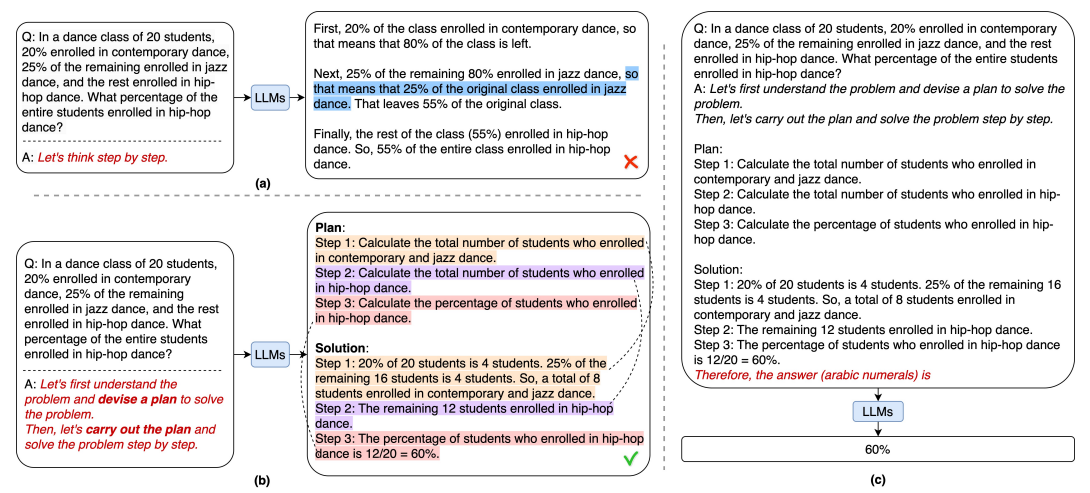
\includegraphics[width=\textwidth]{plan-and-solve}
	\caption{Example inputs and outputs of GPT-3 with (a) Zero-shot-CoT prompting, (b) Plan-and-Solve (PS) prompting, and (c) answer extraction prompting. While Zero-shot-CoT encourages LLMs to generate multi-step reasoning with "Let’s think step by step", it may still generate wrong reasoning steps when the problem is complex. Unlike Zero-shot-CoT, PS prompting first asks LLMs to devise a plan to solve the problem by generating a step-by-step plan and carrying out the plan to find the answer. Source: \textcite{wang2023plan}}
	\label{fig:plan-and-solve}
\end{figure}

\begin{table}[h!]
	\centering
	\begin{tabularx}{\textwidth}{Xcccccc}
		\hline
		\textbf{Method} & \textbf{MultiArith} & \textbf{GSM8k} & \textbf{AddSub} & \textbf{AQUA} & \textbf{SingleEq} & \textbf{SVAMP} \\
		\hline
		Zero-shot-CoT   & 83.8                & 56.4           & 85.3            & 38.9          & 88.1              & 69.9           \\
		PoT             & 92.2                & 57.0           & 85.1            & 43.9          & 91.7              & 70.8           \\
		PS (ours)       & 87.2                & 58.2           & 88.1            & 42.5          & 89.2              & 72.0           \\
		PS+ (ours)      & 91.8                & 59.3           & 92.2            & 46.0          & 94.7              & 75.7           \\
		\hline
	\end{tabularx}
	\caption{Accuracy comparison on math reasoning datasets. Source: \textcite{wang2023plan}}
	\label{tab:ps-math-accuracy}
\end{table}

\begin{table}[h!]
	\centering
	\begin{tabularx}{\textwidth}{Xcc}
		\hline
		\textbf{Method}                & \textbf{CSQA} & \textbf{StrategyQA} \\ \hline
		\textsc{Few-Shot-CoT (Manual)} & 78.3          & 71.2                \\
		\textsc{Zero-shot-CoT}         & 65.2          & 63.8                \\
		\textsc{Zero-shot-PS+}         & \textbf{71.9} & \textbf{65.4}       \\ \hline
	\end{tabularx}
	\caption{Accuracy on commonsense reasoning datasets. Source: \textcite{wang2023plan}}
	\label{tab:commonsense_reasoning}
\end{table}

\begin{table}[h!]
	\centering
	\begin{tabularx}{\textwidth}{Xcc}
		\hline
		\textbf{Method}       & \textbf{Last Letter} & \textbf{Coin Flip} \\ \hline
		Few-Shot-CoT (Manual) & 70.6                 & 100.0              \\
		Zero-shot-CoT         & 64.8                 & 96.8               \\
		Zero-shot-PS+         & \textbf{75.2}        & \textbf{99.6}      \\ \hline
	\end{tabularx}
	\caption{Accuracy on symbolic reasoning datasets. Source: \textcite{wang2023plan}}
	\label{tab:symbolic-reasoning}
\end{table}

Compared to Zero-shot-CoT, which suffers from pitfalls like calculation and missing-step errors, PS+ Prompting has shown to be more effective in addressing these issues~\cite{wang2023plan}.
The experiments with GPT-3 show that PS+ consistently outperforms Zero-shot-CoT and is comparable to 8-shot CoT prompting on math reasoning problems.
Self-consistency (SC)\footnote{It reduces randomness in LLM’s output by generating N reasoning results and determining the final answer by majority voting}\cite{wang2022self} improves performance by generating multiple reasoning paths and determining the final answer by majority voting.
PS+ with SC outperforms PS+ without SC and Zero-shot-CoT with SC\@.

\paragraph{Least-to-Most Prompting}
\label{par:least-to-most}

is a text-based prompting strategy that aims to improve the performance of LLMs on complex reasoning tasks proposed by \textcite{zhou2022least}.
Least-to-most prompting consists of two stages:
\begin{enumerate}
	\item \textbf{Decomposition}: The prompt contains examples demonstrating problem decomposition, followed by the specific question to be decomposed.
	\item \textbf{Sub-problem Solving}: The prompt consists of examples demonstrating sub-problem solving, previously answered subquestions and solutions, and the next question to be answered.
\end{enumerate}
Figure~\ref{fig:least-to-most} illustrates this approach.

\begin{figure}[ht]
	\centering
	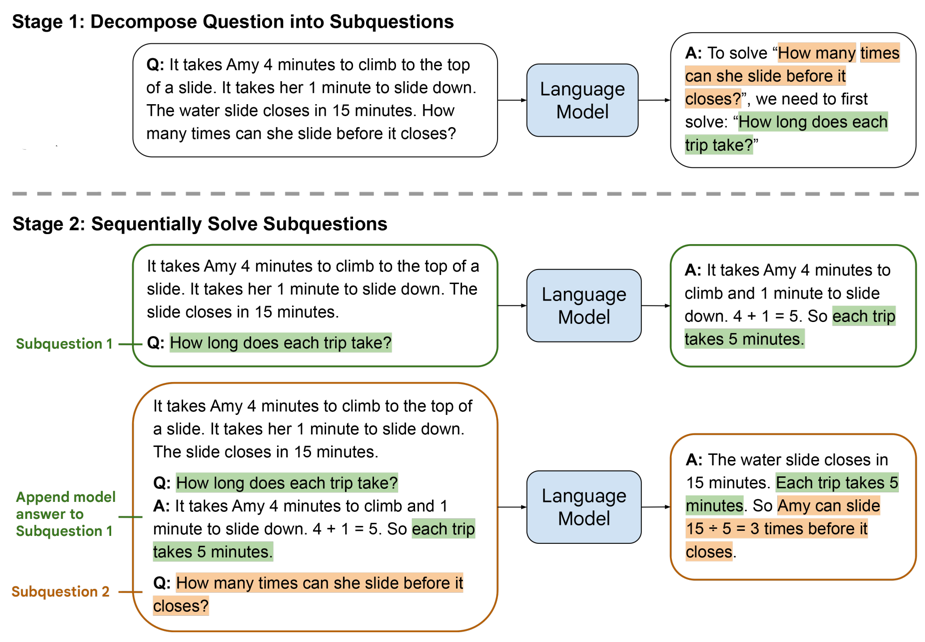
\includegraphics[width=\textwidth]{least-to-most}
	\caption{Least-to-most prompting teaches language models how to solve a complex problem by decomposing it to a series of simpler subproblems. It consists of two sequential stages: (1) decomposition and (2) sequentially solving subproblems. The answer to the second subproblem is built on the answer to the first subproblem. The demonstration examples for each stage’s prompt are omitted in this illustration. Source: \textcite{zhou2022least}}
	\label{fig:least-to-most}
\end{figure}

Least-to-most prompting significantly outperforms Chain-of-Thought prompting on the last-letter-concatenation task\footnote{In this task, each input is a list of words, and the corresponding output is the concatenation of the last letters of the words in the list. For example, "thinking, machine" outputs "ge", since the last letter of "thinking" is "g" and the last letter of "machine" is "e".}~\cite{wei2022chain}, especially on longer lists\footnote{When the testing lists are much longer than the lists in the prompt exemplars.}.
Table~\ref{tab:symbolic} shows the accuracy comparison.

\begin{table}[h!]
	\centering
	\begin{tabularx}{\textwidth}{Xcccccc}
		\hline
		\textbf{Method}    & \textbf{Length 4} & \textbf{Length 6} & \textbf{Length 8} & \textbf{Length 10} & \textbf{Length 12} \\
		\hline
		Standard Prompting & 0.0               & 0.0               & 0.0               & 0.0                & 0.0                \\
		Chain-of-Thought   & 84.2              & 69.2              & 50.2              & 39.8               & 31.8               \\
		Least-to-Most      & 94.0              & 88.4              & 83.0              & 76.4               & 74.0               \\
		\hline
	\end{tabularx}
	\caption{Accuracies of different prompting methods on the last-letter-concatenation task. Source: \textcite{zhou2022least}}
	\label{tab:symbolic}
\end{table}

Least-to-most prompting also achieves 99.7\% accuracy on the SCAN\footnote{it is probably the most popular benchmark for evaluating compositional generalization. It requires mapping natural language commands to action sequences~\cite{lake2018generalization}.} compositional generalization benchmark with only 14 exemplars, compared to 16\% with Chain-of-Thought prompting.
Table~\ref{tab:compositional} shows the accuracy comparison.
Least-to-most improves performance on GSM8k and DROP benchmarks, particularly for problems requiring multiple solving steps.
Table~\ref{tab:math} shows the accuracy comparison.

\begin{table}[h!]
	\centering
	\begin{tabularx}{\textwidth}{Xccc}
		\hline
		\textbf{Method}    & \textbf{Code-davinci-002} & \textbf{Text-davinci-002} & \textbf{Code-davinci-001} \\
		\hline
		Standard Prompting & 16.7                      & 6.0                       & 0.4                       \\
		Chain-of-Thought   & 16.2                      & 0.0                       & 0.0                       \\
		Least-to-Most      & 99.7                      & 76.0                      & 60.7                      \\
		\hline
	\end{tabularx}
	\caption{Accuracies of different prompting methods on the SCAN benchmark. Source: \textcite{zhou2022least}}
	\label{tab:compositional}
\end{table}
\begin{table}[h!]
	\centering
	\begin{tabularx}{\textwidth}{Xccc}
		\hline
		\textbf{Method}    & \textbf{Non-football (DROP)} & \textbf{Football (DROP)} & \textbf{GSM8k} \\
		\hline
		Zero-Shot          & 43.86                        & 51.77                    & 16.38          \\
		Standard Prompting & 58.78                        & 62.73                    & 17.06          \\
		Chain-of-Thought   & 74.77                        & 59.56                    & 60.87          \\
		Least-to-Most      & 82.45                        & 73.42                    & 62.39          \\
		\hline
	\end{tabularx}
	\caption{Accuracies of different prompting methods on GSM8k and DROP benchmarks. Source: \textcite{zhou2022least}}
	\label{tab:math}
\end{table}

Least-to-most prompting effectively generalizes to more complex problems than those seen in the prompts.
This approach can be combined with other prompting techniques, such as chain-of-thought and self-consistency, to further enhance performance.


\paragraph{DECOMP}
\label{par:decomp}
is a text-based prompting strategy that decomposes complex tasks into simpler subtasks and generates a plan to solve the task, similar to Least-to-Most prompting.
The core idea of Decomposed Prompting involves dividing a complex task into multiple simpler subtasks.
Each subtask is addressed separately using LLMs, and their results are then combined to produce the final outcome.
Tasks are decomposed based on their inherent structure.
For instance, a question-answering task might be split into subtasks involving information retrieval, comprehension, and synthesis.
By focusing on these individual components, the model can process each step more effectively.

\begin{figure}[h!]
	\centering
	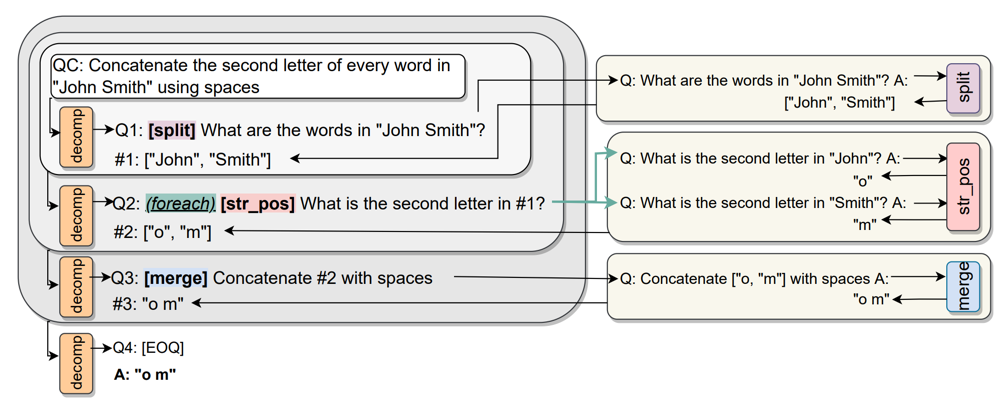
\includegraphics[width=0.8\textwidth]{decomp}
	\caption{The DECOMP framework. Source: \textcite{khot2022decomposed}}
	\label{fig:decomp}
\end{figure}

In DECOMP, the core is a decomposer LLM that tries to solve a complex task by generating a prompting program $P$.
Each step of $P$ directs a simpler sub-query to a function in an auxiliary set of sub-task functions F available to the system.
Given a query $Q$ whose answer is $A$, the program $P$ is a sequence of the form $((f_1, Q_1, A_1), \ldots ,(f_k, Q_k, A_k))$
where $A_k$ is the final answer predicted by $P$ and $Q_i$ is a sub-query directed to the sub-task function $f_i \in F$.
$P$ is executed by a high-level imperative controller, which passes the inputs and outputs between the decomposer and sub-task handler until a stopping condition in $P$ is met and the final output is obtained.
Using a software engineering analogy, the decomposer defines the top-level program for the complex task using interfaces to simpler sub-task functions.
The sub-task handlers serve as modular, debuggable, and upgradable implementations of these simpler functions, akin to a software library.
Specialized prompts are designed for each subtask, guiding the LLM to focus on specific aspects of the problem.
This involves crafting precise and contextually relevant prompts that direct the model's attention to the desired task component.

Extensive experiments demonstrate the efficacy of Decomposed Prompting.
Key benchmarks and datasets were utilized to evaluate the performance gains achieved through this approach (Figure~\ref{fig:decomp-results}).

\begin{figure}[h!]
	\centering
	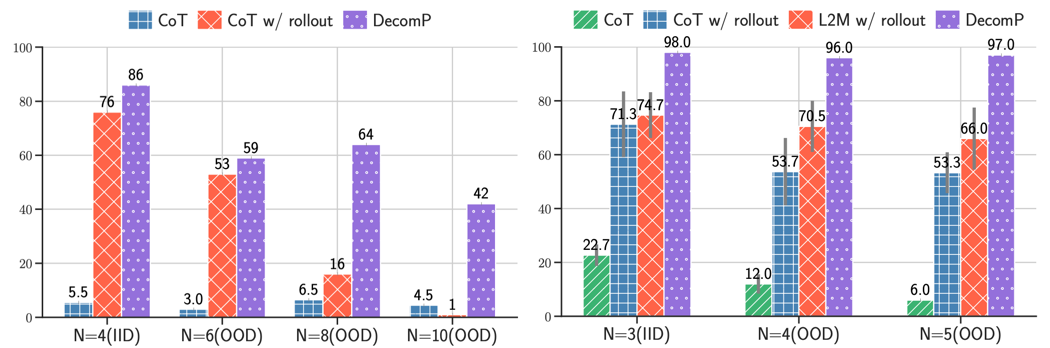
\includegraphics[width=0.8\textwidth]{decomp-results}
	\caption{On the left: Exact Match results on the k-th letter concatenation task (k=3) using space as a delimiter with different numbers of words in the input. On the right: Exact Match results on reversing sequences. Incorporating CoT in DECOMP greatly increases the ability of the model to generalize to new sequence lengths Source: \textcite{khot2022decomposed}}
	\label{fig:decomp-results}
\end{figure}

\paragraph{Program-Aided Language Models (PALMs)}
\label{par:program-aided-language-models}

are a new class of code-based language models that use the LLM to read natural language problems and generate programs as the intermediate reasoning steps, but they offload the solution step to a runtime such as a Python interpreter.
These models are designed to perform complex reasoning tasks that require structured knowledge and logical reasoning, such as mathematical word problems, symbolic reasoning, and program synthesis.
Despite LLMs seeming to be adept at CoT prompting, LLMs often make mathematical and logical errors, even though the problem is decomposed correctly into intermediate reasoning steps~\cite{gao2022pal}.

\textsc{PaL} is a model that belongs to this new class of models.
It generates programs that can be executed by a Python interpreter and uses the program's output as the final answer.
\begin{figure}[h!]
	\centering
	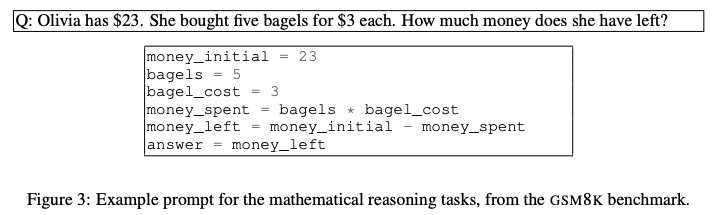
\includegraphics[width=0.8\textwidth]{pal-math}
	\caption{Example prompt for the mathematical reasoning tasks from the GSM8k benchmark. Source: \textcite{gao2022pal}}
	\label{fig:pal-math}
\end{figure}
\begin{figure}[h!]
	\centering
	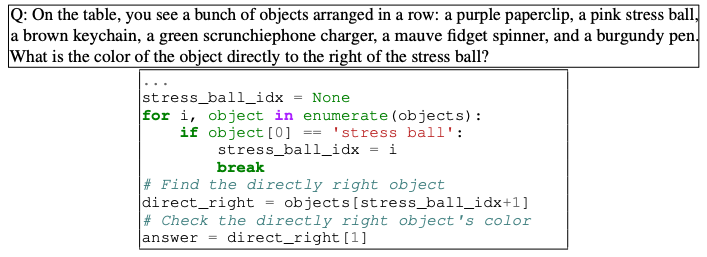
\includegraphics[width=0.8\textwidth]{pal-colored}
	\caption{An example for a \textsc{PaL} prompt in the \textsc{Colored Objects} task. Source: \textcite{gao2022pal}}
	\label{fig:pal-colored}
\end{figure}
\textsc{PaL} has been shown to outperform much larger LLMs using CoT (e.g., PaLM-540B) on mathematical word problems and symbolic reasoning tasks~\cite{gao2022pal} as shown in Table~\ref{tab:pal-math}.
\begin{table}[h!]
	\centering
	\tiny
	\begin{tabularx}{\textwidth}{XXXXXXXXXX}
		\hline
		\textbf{Model}                           & \textbf{GSM8k} & \textbf{GSM-HARD} & \textbf{SVAMP} & \textbf{ASDIV} & \textbf{SINGLEEQ} & \textbf{SINGLEOP} & \textbf{ADDSUB} & \textbf{MULTIARITH} \\ \hline
		\textsc{Direct}\textsubscript{Codex}     & 19.7           & 5.0               & 69.9           & 74.0           & 86.8              & 93.1              & 90.9            & 44.0                \\
		\textsc{CoT}\textsubscript{UL2-20B}      & 4.1            & -                 & 12.6           & 16.9           & -                 & -                 & 18.2            & 10.7                \\
		\textsc{CoT}\textsubscript{LAMDA-137B}   & 17.1           & -                 & 39.9           & 49.0           & -                 & -                 & 52.9            & 51.8                \\
		\textsc{CoT}\textsubscript{Codex}        & 65.6           & 23.1              & 74.8           & 76.9           & 89.1              & 91.9              & 86.0            & 95.9                \\
		\textsc{CoT}\textsubscript{PaLM-540B}    & 56.9           & -                 & 79.0           & 73.9           & 92.3              & 94.1              & 91.9            & 94.7                \\
		\textsc{CoT}\textsubscript{Minerva} 540B & 58.8           & -                 & 79.4           & 79.6           & 96.1              & 94.6              & 92.5            & 99.2                \\
		\textsc{PaL}                             & \textbf{72.0}  & \textbf{61.2}     & \textbf{79.4}  & \textbf{79.6}  & \textbf{96.1}     & \textbf{94.6}     & \textbf{92.5}   & \textbf{99.2}       \\ \hline
	\end{tabularx}
	\caption{Problem solve rate (\%) on mathematical reasoning datasets. The highest number on each task is in \textbf{bold}. The results for DIRECT and PaLM-540B are from \textcite{wei2022chain}, the results for LAMDA and UL2 are from \textcite{wang2022self}, the results for Minerva are from \textcite{lewkowycz2022minerva}. PAL ran on each benchmark 3 times and reported the average. Source: \textcite{gao2022pal}.}
	\label{tab:pal-math}
\end{table}
\textsc{PaL} is even more effective with respect to other LLMs when tested on the GSM-HARD dataset -- a version of GSM8k contains larger numbers (i.e., up to 7 digits).
Other interesting results come from symbolic reasoning tasks from BIG-Bench Hard: the \textsc{Colored Objects}\footnote{It requires answering questions about coloured objects on a surface} and the \textsc{Penguins}\footnote{It requires to answer a question about the attributes of the penguins on a table (e.g., "how many penguins are less than 8 years old?"). This task describes dynamics as well since the penguins can be added or removed.} tasks as shown in Table~\ref{tab:pal-symbolic}.
\begin{table}[h!]
	\centering
	\small
	\begin{tabularx}{\textwidth}{XXXXXXX}
		\hline
		\textbf{Model}                         & \textbf{COLORED                                                                 \newline OBJECT} & \textbf{PENGUINS} & \textbf{DATE} & \textbf{REPEAT \newline COPY} & \textbf{OBJECT COUNTING} \\ \hline
		\textsc{Direct}\textsubscript{Codex}   & 75.7                                                                                             & 71.1              & 49.9          & 81.3                          & 37.6                     \\
		\textsc{CoT}\textsubscript{LAMDA-137B} & -                                                                                                & -                 & 26.8          & -                             & -                        \\
		\textsc{CoT}\textsubscript{PaLM-540B}  & -                                                                                                & 65.1              & 65.3          & -                             & -                        \\
		\textsc{CoT}\textsubscript{Codex}      & 86.3                                                                                             & 79.2              & 64.8          & 68.8                          & 73.0                     \\
		\textsc{PAL}\textsubscript{Codex}      & \textbf{95.1}                                                                                    & \textbf{93.3}     & \textbf{76.2} & \textbf{90.6}                 & \textbf{96.7}            \\ \hline
	\end{tabularx}
	\caption{Solve rate on three symbolic reasoning datasets and two algorithmic datasets. In all datasets, PAL achieves a much higher accuracy than chain-of-thought. Results with closed models LAMDA-137B and PaLM-540B are included if available to public \textcite{wei2022chain, suzgun2022challenging}. Source: \textcite{gao2022pal}.}
	\label{tab:pal-symbolic}
\end{table}
\textcite{gao2022pal} have shown that \textsc{PaL} is not limited to LMs of code, but it can work with LMs that were mainly trained for natural language if they have a sufficiently high coding ability, and benefits come from the synergy between the Python prompt and the interpreter.
\textsc{PaL} avoids inaccuracy on arithmetic tasks and incorrect reasoning by offloading the calculations and some of the reasoning to a Python interpreter, which is correct by design, giving the the right program.

\paragraph{SELF-PLANNING}
\label{par:self-planning}

is a code-generation strategy using a planning-based approach.
In this case, the planning is executed prior to the actual code generation, and the plan is generated by the LLM itself.
In the first stage, the planning phase, the LLM is prompted to abstract and decompose the intent to obtain a plan for guiding code generation using few-shot prompting.
The prompt $C$ is designed as $k$ examples\footnote{Note that $k$ is a fairly low number.} concatenated together
\begin{equation}
	C \stackrel{\Delta}{=} \left\langle x^e_1 \cdot y^e_1 \right\rangle \bigparallel \left\langle x^e_2 \cdot y^e_2 \right\rangle \bigparallel \ldots \bigparallel \left\langle x^e_k \cdot y^e_k \right\rangle
	\label{eq:self-planning-eq}
\end{equation}
where each example $\left\langle x^e_i \cdot y^e_i \right\rangle$ consists of the example intent $x^e_i$ and its associated plan $y^e_i$ to demonstrate the planning task.
During inference, the test-time intent $x$ will be concatenated after the prompt, and $C \bigparallel x$ will be fed into the LLM $M$, which will attempt to do planning for the test-time intent.
The output of the LLM is the test-time plan $y$ for the test-time intent $x$.

\begin{figure}[h!]
	\centering
	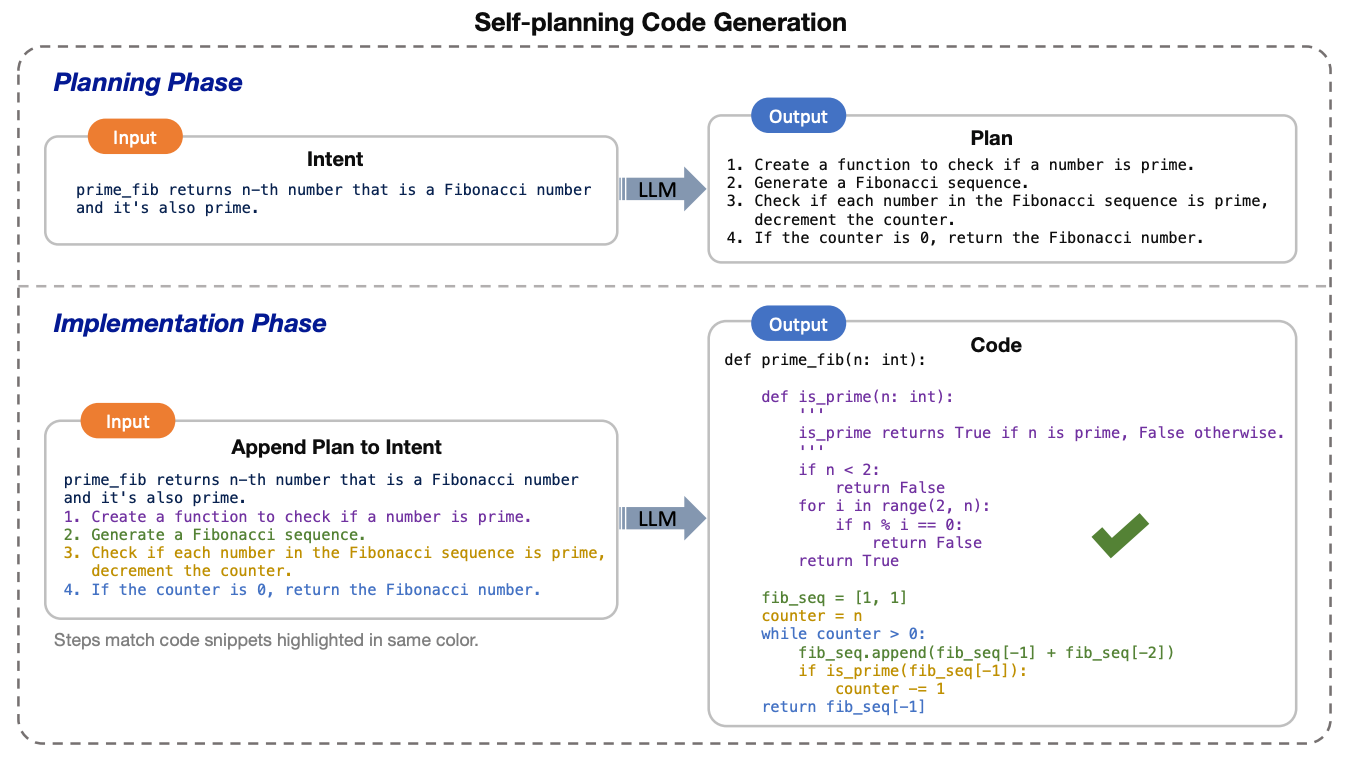
\includegraphics[width=\textwidth]{self-planning}
	\caption{Self-planning generation phases (i.e., planning phase and implementation phase). Source: \textcite{jiang2024selfplanning}}
	\label{fig:self-planning}
\end{figure}

In the second stage, the implementation phase, the plan generated in the first stage guides the code generation.
The plan $y$ is concatenated with intent $x$ and fed into the LLM $M$ to generate the code $z$.
The above two stages can be formalized as
\begin{equation}
	P(z|x, C) = \sum_{\hat{y}}{P(z|\hat{y}, x, C) \cdot P(\hat{y}|x, C)},\\
	\propto P(z|y, x, C) \cdot P(y|x, C)
	\label{eq:self-planning-all}
\end{equation}
where $\hat{y}$ is any of all possible plans, and $y$ denotes one of the plans generated by the LLM in the first stage.
\textcite{jiang2024selfplanning} further simplifies the above equation by adopting the plan with the highest probability as $y$. Thus, the final equation becomes
\begin{equation}
	P(z|x, C) \stackrel{\Delta}{=} \underbrace{P(z|y, x, C)}_\text{Implementation phase} \cdot \underbrace{P(y|x, C)}_\text{Planning phase}
	\label{eq:self-planning-final}
\end{equation}

Benchmarking against various LLMs pre-trained on code, such as CodeGeex (13B)~\cite{zheng2023codegeex}, CodeGen-Mono (16.1B)~\cite{nijkamp2022codegen}, and PaLM Coder (560B)~\cite{chung2022scaling}, reveals that SELF-PLANNING significantly enhances performance across public code generation datasets.
This improvement is observed when comparing SELF-PLANNING with other prompting methods, including Direct, Code Chain-of-Thought (CoT), and Few-shot approaches.
Comparing the effectiveness of SELF-PLANNING relative to model size, it is evident that SELF-PLANNING impact is more pronounced with larger models.
As the model size reaches 13B, LLMs' performance in code generation tasks begins to exhibit emerging ability, but self-planning ability is still relatively low.
Experiments show that incorporating code training data and RLHF can enhance the model’s self-planning capabilities and increase its size.

\subsubsection{Feedback and plan refinement}
\label{subsubsec:feedback}

Feedback is an essential component in the plan-based reasoning paradigm, as it allows the planner to refine the plan based on the feedback from the environment following the "\textit{planning-execution-refinement}" loop.
Feedback sources are categorized into internal and external, based on their origin relative to the LLM-based planner.

\textbf{Internal Feedback:} Here, the LLM itself acts as a source of feedback.
One common method is to assess the effectiveness of generated plans through structured prompts.
For instance, \textcite{hao2023reasoning} evaluates the success potential of various plans by estimating their likelihood of achieving the desired outcome, while Tree of Thoughts employs a comparative voting mechanism among different plans.
Additionally, LLMs can refine their feedback using intermediate outcomes from plan execution, such as in Reflexion, where sparse outcomes like success or failure are translated into detailed, actionable feedback.
This feedback is then preserved in the LLM’s long-term memory to enhance future planning.

\textbf{External Feedback:} Beyond the LLM, external tools and environments contribute feedback as well.
Tools such as code interpreters in programming tasks offer immediate error feedback, while models like stable diffusion in multimodal tasks provide visual feedback.
Virtual environments like Minecraft offer a rich, interactive backdrop for feedback through immersive experiences.
Moreover, projects like Generative Agents investigate the dynamics of multi-agent systems in simulated settings, where agents derive feedback from both environmental interactions and inter-agent communication.

Regarding the plan refinement, the three main approaches are summarized in the next paragraphs.

\paragraph{Reasoning.}
\label{par:reasoning}

When the feedback data from the environment is not directly suitable to be utilized by LLMs for plan refinement, some work adds the explicit reasoning process to extract critical information from feedback~\cite{chen2023chatcot, yao2022react}.
React prompts LLMs with demonstrations to generate reasoning traces over feedback.
Human intelligence uniquely integrates task-oriented actions with verbal reasoning or "inner speech, " significantly contributing to cognitive functions like self-regulation and working memory management.
For example, in the kitchen, a person might verbally strategize their next steps in a recipe ("Now that everything is cut, I should heat up the pot of
water"), adapt to missing ingredients ("I don’t have salt, so let me use soy sauce and pepper instead"), or seek additional information online to enhance their cooking process.
This ability to blend action with analytical thinking enables humans to swiftly learn new tasks and make robust decisions, even in novel or uncertain situations.
\begin{figure}[h!]
	\centering
	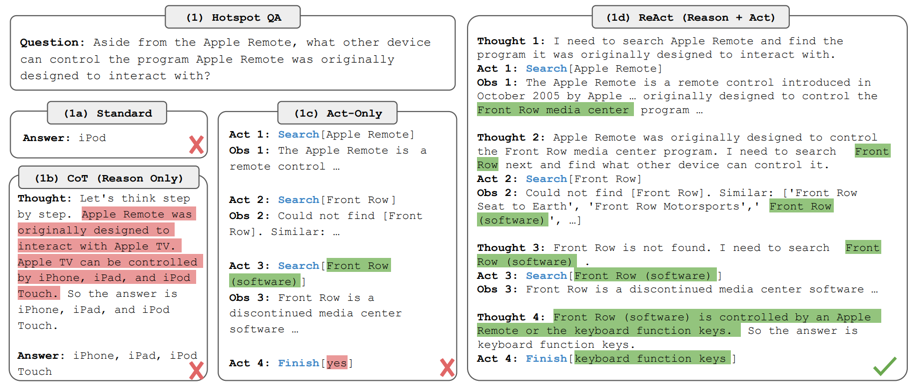
\includegraphics[width=\textwidth]{react}
	\caption{(1) Comparison of 4 prompting methods, (a) Standard, (b) Chain-of-thought (CoT, Reason Only), (c) Act-only, and (d) ReAct (Reason+Act), solving a HotpotQA \cite{yang2018hotpotqa} question. Source: \textcite{chen2023chatcot}}
	\label{fig:react}
\end{figure}
React has been widely used in autonomous agent projects, such as AutoGPT, which can automatically reason over the observed feedback to revise the initial plan for solving various user requests.
However, these approaches typically fix the order of reasoning and planning.
\begin{figure}[h!]
	\centering
	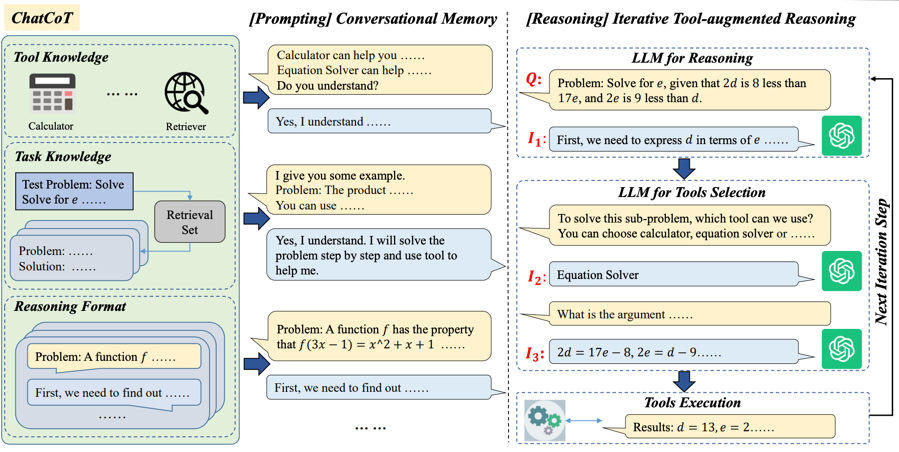
\includegraphics[width=\textwidth]{chatcot}
	\caption{ChatCoT strategy illustrated to solve a mathematical problem. The conversational knowledge memory is initialized to provide tools, task and reasoning format knowledge. Then, the tool-augmented reasoning step is iterated multiple times to perform step-by-step reasoning until the answer is obtained. Source: \textcite{chen2023chatcot}}
	\label{fig:chatcot}
\end{figure}

ChatCoT supports flexible switching between the two processes, unifying the tool-augmented CoT reasoning framework into a multi-turn conversation between the LLM-based task planner and the tool-based environment.
At each turn, the LLM can freely interact with tools when needed; otherwise, it performs the reasoning by itself.

\paragraph{Backtracking.}
\label{par:backtracking}

Initial planning techniques primarily focused on progressing with forward actions within an existing plan, often resulting in locally optimal strategies based on short-term assessments.
To address this limitation, the Tree of Thoughts approach~\cite{yao2023tree} introduces the capability for backtracking through search techniques such as breadth-first and depth-first searches, enabling more comprehensive global planning strategies.
This method iteratively refines the plan by returning to previous decision points and exploring alternative paths as depicted in Figure~\ref{fig:tree-of-thoughts}.

\begin{figure}[h!]
	\centering
	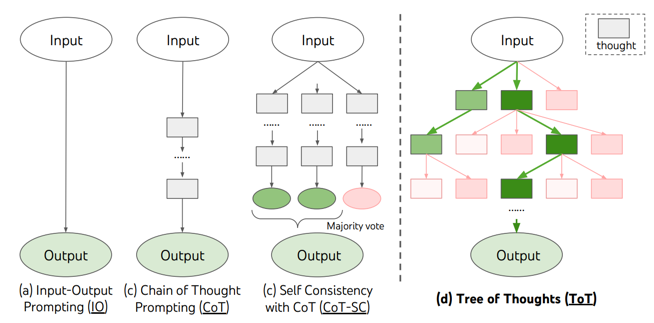
\includegraphics[width=\textwidth]{tree-of-thoughts}
	\caption{Diagram demonstrating various problem-solving methodologies using LLMs. Each rectangle represents a distinct thought, forming an integral step towards resolving a problem. Source: \textcite{yao2023tree}}
	\label{fig:tree-of-thoughts}
\end{figure}

In developing such a method, \textcite{yao2023tree} revisits foundational artificial intelligence and cognitive science principles, framing problem-solving as navigating a tree-like combinatorial space.
Within this framework, \textcite{yao2023tree} introduced three novel challenges aimed at pushing the boundaries of state-of-the-art models such as GPT-4: the Game of 24\footnote{The Game of 24 is a mathematical challenge where the objective is to manipulate four numbers using basic arithmetic operations \code{$+-\times\div$} to achieve a result of 24. For instance, from the numbers \code{4, 9, 10, 13}, one possible solution could be \code{$(10 - 4) \times (13 - 9) = 24$}.}, Creative Wiring\footnote{In the Creative Wiring task, participants are given four random sentences and must craft a coherent narrative consisting of four paragraphs, each concluding with one of the provided sentences. This task tests creative synthesis and advanced planning.}, and Crosswords\footnote{A $5\times5$ mini crosswords task is a harder search problem involving natural language. The goal is not to solve the problem since it can be solved with specialized NLP pipelines but to explore the limit of LM as a general-purpose solver.}.
These tasks necessitate a blend of deductive, mathematical, commonsense, and lexical reasoning skills, along with sophisticated systematic planning or searching capabilities.
The Tree of Thoughts model demonstrates its versatility and efficacy across these diverse tasks by supporting varied levels of thought processes, multiple thought generation and assessment methods, and adaptable search algorithms tailored to the specifics of each challenge.

Furthermore, some studies~\cite{hao2022structured, wang2023describeexplainplanselect} utilize feedback signals to revise the entire plan since the initial plan generated by the LLM is often imperfect.
For example, DEPS\footnote{Describe, Explain, Plan, Select}~\cite{wang2023describeexplainplanselect} selects a better plan according to feedback signals, while TIP\footnote{Text-Image Prompting}~\cite{lu2023multimodal} adds feedback signals to prompts for the LLM-based planner to revise each step in the initial plan.

DEPS has been tested on Minecraft, an open world with abundant object types and complex dependencies and relations.
As a result, ground-truth plans typically involve a long sequence of sub-goals with strict dependencies (e.g., obtaining a diamond requires 13 sub-goals with strict dependencies).
Another challenge in an open-ended world is the feasibility of the produced plans.
For example, the fastest way to craft a bed in Minecraft is to slaughter a sheep to obtain wool, which can be used to craft beds or collect beds from a village.
However, since no sheep or village is reachable by the agent within 3 minutes of gameplay, to craft a bed efficiently, the agent should choose to slaughter a spider and use materials (e.g., string) it drops to craft wool, and then a bed.
\begin{figure}[h!]
	\centering
	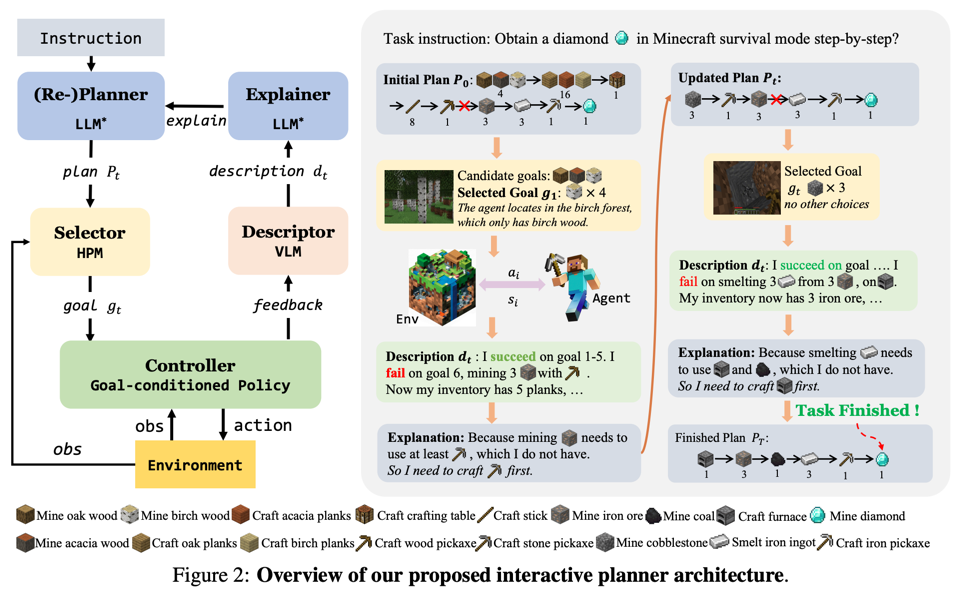
\includegraphics[width=\textwidth]{deps}
	\caption{Overview of the DEPS interactive plannet architecture. Source: \textcite{wang2023describeexplainplanselect}}
	\label{fig:deps}
\end{figure}
The key to solving the first challenge is effectively adjusting the generated plan upon a failure.
When the controller fails to complete a sub-goal, a descriptor will summarize the current situation as text and send it back to the LLM-based planner.
Then, prompt the LLM as an explainer to locate the errors in the previous plan.
Finally, a planner will refine the plan using information from the descriptor and explainer.
To improve the feasibility of generated plans conditioned on the current state, which is the second identified challenge, \textcite{wang2023describeexplainplanselect} use a learned goal-selector to choose the most accessible sub-task based on the proximity to each candidate sub-goal.
Developing multi-task agents that can accomplish a vast and diverse suite of tasks in complex domains has been viewed as one of the key milestones towards generally capable artificial intelligence.

\paragraph{Memorization}
\label{par:memorization}

Long-term memory is a crucial component in the planning process. It allows models to store and retrieve information from past experiences, in addition to the short-term memory capabilities provided by in-context learning (ICL) in large language models (LLMs).
Reflexion~\cite{shinn2023reflexion} introduces an innovative framework that enhances language agents through linguistic feedback rather than weight updates.
Reflexion agents reflect verbally on task feedback, maintaining reflective text in an episodic memory buffer to improve decision-making in subsequent trials.
This process mirrors how humans iteratively learn complex tasks by reflecting on previous failures to develop improved strategies for future attempts.

\begin{figure}[h!]
	\centering
	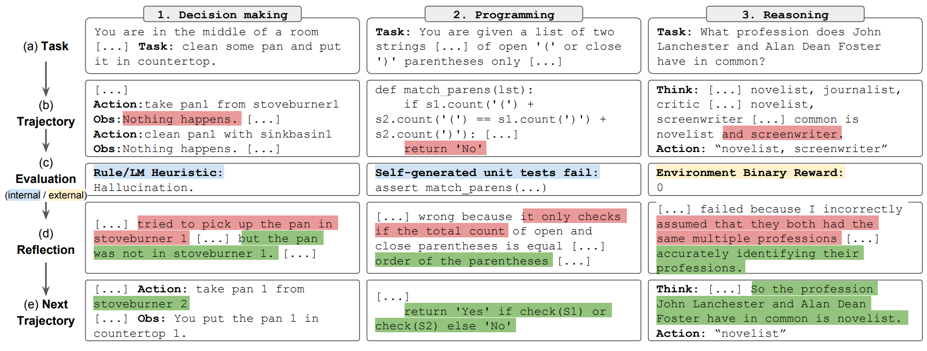
\includegraphics[width=\textwidth]{reflexion}
	\caption{Reflexion works on decision-making, programming, and reasoning tasks. Source: \textcite{shinn2023reflexion}}
	\label{fig:reflexion}
\end{figure}

Reflexion can incorporate various types (scalar values or free-form language) and sources (external or internally simulated) of feedback signals, significantly improving performance over a baseline agent across diverse tasks such as sequential decision-making, coding, and language reasoning.

\begin{figure}[h!]
	\centering
	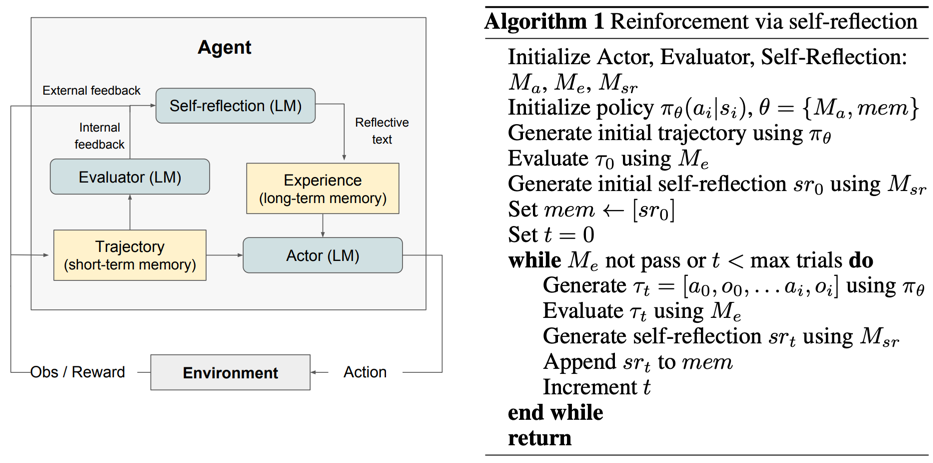
\includegraphics[width=\textwidth]{reflexion-alg}
	\caption{(a) Diagram of Reflexion. (b) Reflexion reinforcement algorithm. Source: \textcite{shinn2023reflexion}}
	\label{fig:reflexion-alg}
\end{figure}

The Reflexion framework consists of four main components: the Actor, the Evaluator, the Self-Reflection model, and the memory.
The Actor, built upon an LLM, is specifically prompted to generate necessary text and actions based on state observations.
The Evaluator assesses the quality of the Actor's outputs by computing a reward score that reflects performance within the given task context.
The Self-Reflection model, also instantiated as an LLM, generates verbal self-reflections to provide valuable feedback for future trials.
Core components of the Reflexion process are the notion of short-term and long-term memory.
At inference time, the Actor conditions its decisions on short and long-term memory, similar to the way that humans remember fine-grain recent details while also recalling distilled important experiences from long-term memory.
In the RL setup, the trajectory history serves as the short-term memory, while outputs from the Self-Reflection model are stored in long-term memory.
These two memory components work together to provide specific context but are also influenced by lessons learned over several trials, which is a key advantage of Reflexion agents over other LLM action choice works.
Given a sparse reward signal, such as a binary success status (success/fail), the current trajectory, and its persistent memory \(mem\), the self-reflection model generates nuanced and specific feedback.
This feedback, which is more informative than scalar rewards, is then stored in the agent’s memory \(mem\).
For example, in a multi-step decision-making task, if the agent receives a failure signal, it can infer that a specific action \(a_i\) led to subsequent incorrect actions \(a_{i+1}\) and \(a_{i+2}\).
The agent can then verbally state that it should have taken a different action, \(a_i\), which would have resulted in correct actions \(a_{i+1}\) and \(a_{i+2}\), and store this experience in its memory.
In subsequent trials, the agent can leverage its past experiences to adapt its decision-making approach at time \(t\) by choosing action \(a_i\).
This iterative process of trial and error, self-reflection, and persisting memory enables the agent to rapidly improve its decision-making ability in various environments by utilizing informative feedback signals.
For instance, Reflexion achieves a 91\% pass@1 accuracy on the HumanEval coding benchmark, surpassing the previous state-of-the-art GPT-4, which achieves 80\%.

\begin{figure}[h!]
	\centering
	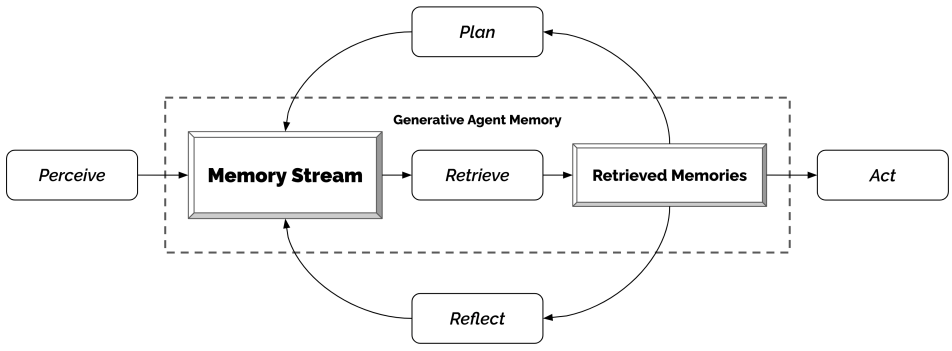
\includegraphics[width=\textwidth]{generative-agent}
	\caption{Generative agent architecture. Agents perceive their environment, and all perceptions are saved in a comprehensive record of the agent’s experiences called the memory stream. Based on their perceptions, the architecture retrieves relevant memories and uses those retrieved actions to determine an action. These retrieved memories are also used to form longer-term plans and create higher-level reflections, both of which are entered into the memory stream for future use. Source: \textcite{park2023generativeagentsinteractivesimulacra}}
	\label{fig:generative-agents}
\end{figure}

Generative agents~\cite{park2023generativeagentsinteractivesimulacra} are another example of models that leverage memory to improve planning where a sandbox environment is populated with 25 agents that focus on the ability to create a small, interactive society of agents inspired by games such as The Sims.
In particular, the generative agents leverage a memory stream mechanism for action planning and reflection, simulating human-like decision behaviour.
The memory stream is a long-term memory module that records a comprehensive list of the agent’s experiences in natural language.
The reflection and the planning components synthesize memories into higher-level inferences over time, enabling the agent to draw conclusions
about itself and others, and translates those conclusions and the current environment into high-level action plans recursively, as shown in Figure~\ref{fig:generative-agents}.

Other studies~\cite{sun2023adaplanner, wang2023voyager} have also explored using memory called skill library mechanism to store successful plans, which can be reused and synthesized as complex plans for new tasks.
AdaPlanner~\cite{sun2023adaplanner} uses skill memory as a repository, archiving past successful plans and their respective interactions with the environment.
If the agent encounters a task resembling the skills stored in memory, these skills can serve as few-shot exemplars in the LLM agent’s prompt.
This feature improves not only sample efficiency but also reliability for future planning.
\begin{figure}[h!]
	\centering
	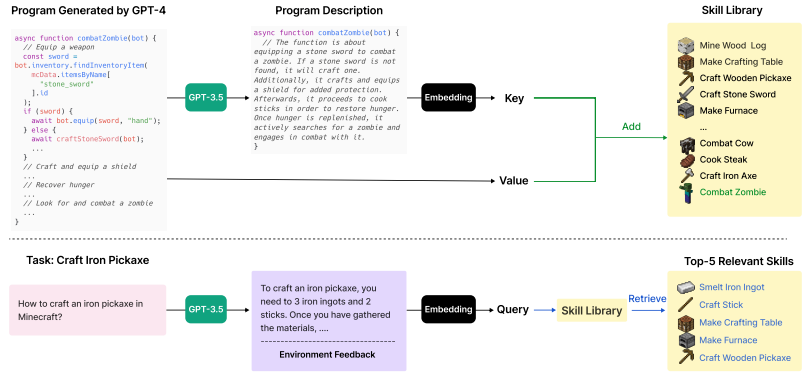
\includegraphics[width=\textwidth]{skill-library}
	\caption{Adding and retrieving skills from the skill library in Voyager. Source: \textcite{sun2023adaplanner}}
	\label{fig:skill-library}
\end{figure}
To implement the long-term memory, \textcite{wang2023voyager, wang2021milvus} proposes tools like vector databases, which can be used to store plans or feedback into high-dimensional vectors.\footnote{A vector database is a type of database engineered specifically for handling vector data, which are arrays of numbers or embeddings representing various types of data objects.
	These databases are designed to efficiently store, manage, and perform operations on vectors, which are often used to represent images, text, or other complex data types in a form suitable for machine learning models and similarity search operations.
	Vector databases excel in handling similarity searches, which involve finding vectors closest to a given vector.
	They are optimized to store and query high-dimensional data efficiently.}
\begin{figure}[h!]
	\centering
	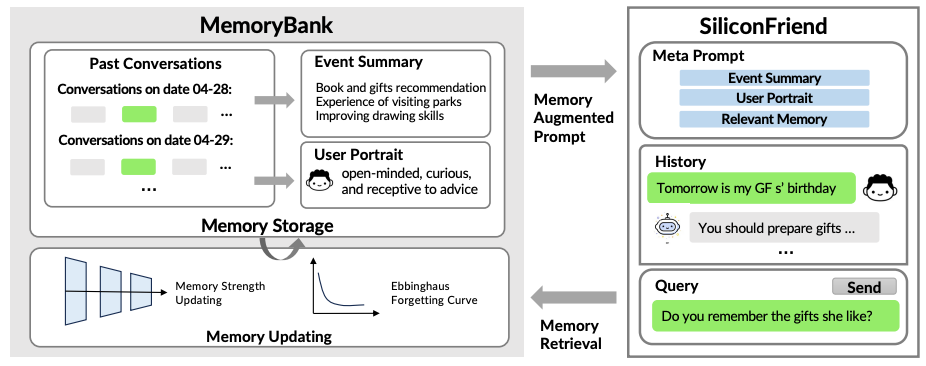
\includegraphics[width=\textwidth]{memorybank}
	\caption{Overview of MemoryBank. The memory storage stores past conversations, summarized events and user portraits, while the memory updating mechanism updates the memory storage. Memory retrieval recalls relevant memory. Source: \textcite{zhong2023memorybankenhancinglargelanguage}}
	\label{fig:memorybank}
\end{figure}
MemoryBank~\cite{zhong2023memorybankenhancinglargelanguage} incorporates a memory updating mechanism inspired by the Ebbinghaus Forgetting Curve theory.\footnote{The Ebbinghaus Forgetting Curve is a psychological theory that describes how information is lost over time when there is no attempt to retain it.
	It shows that humans tend to halve their memory of newly learned knowledge in a matter of days or weeks unless they consciously review the learned material.}
This mechanism allows the model to forget less relevant information and retain more important information based on time elapsed and the relative relevance of the information, thereby offering a human-like memory management system.


